\documentclass[../main/thesis]{subfiles}

% Overleaf graphics path
\graphicspath{{thesis/model_development/figures/}}

% \graphicspath{{/home/arefk/uio/MScThesis_AreKvanum2022_SeaIceML/thesis/model_development/figures/}}
\begin{document}

\section{Model development}
\label{sec:developing a unet}
This section will cover the implementation of the U-Net architecture, as well as related processes such as data preparation and writing a custom dataloader. Furthermore, this section will present intermediate results obtained during development to highlight technical decisions made as well as their consequence for model performance. Decisions made will be highlighted from a statistical point of view, and when relevant they will also be explored in a context of the underlying physics.

\subsection{Data preprocessing}
The deep learning system can be disassembled into two parts, a dataloader followed by the deep learning model itself. The dataloader structures already preprocessed data that are then provided to the deep learning model during training. However, the predictors from a sample are from different datasets provided on different spatial grids and temporal frequency. Thus, preliminary computations are required in order to extract the desired spatiotemporal information from each predictor onto a common grid. Since the preparatory work on the predictors only need to be done once, the preprocessing is performed in advance of the training process. The following sections describes how the preprocessing is performed on the different datasets.

An overview of the data pipeline and workflow is described in Figure \ref{fig:data_pipeline}. As can be seen from Figure \ref{fig:data_pipeline}, a sample is constructed from a recent sea ice chart \citep{Dinessen2020}, the computed sea ice concentration trend over a set amount of previous days from OSI SAF SSMIS observations \citep{Tonboe2017}, recent AROME Arctic \citep{Mueller2017} 2-meter temperature and wind forecasts as well as a land-sea mask, which comes from AROME Arctic. 

\begin{figure}
    \centering
    % \includestandalone[width=.865\textwidth]{/home/arefk/uio/MScThesis_AreKvanum2022_SeaIceML/thesis/model_development/figures/pipeline}
    \includestandalone[width=.865\textwidth]{thesis/model_development/figures/pipeline}
    \caption{\label{fig:data_pipeline} Workflow figure providing an overview of the data pipeline. Data are sampled from four sources (Sea Ice Charts, OSI SAF SSMIS, AROME Arctic and a Land Sea Mask), preprocessed and merged into a single sample. The sample is fed into the network together with an associated sea ice chart which is the target variable. The predicted sea ice chart is compared against the ground truth sea ice chart, and their binary cross entropy error is propagated backwards throughout the network, which constitutes a step in the training loop.}
\end{figure}

\subsubsection{Regridding data}
\label{sec:regrid}
All input data loaded into the U-Net are on the AROME Arctic projection with a 1km spatial resolution and cover the same domain as required by the input layer of the U-Net architecture \citep{Ronneberger2015}. For geographic data, this requirement implies that all data used for training, validation or testing of the deep learning system has to be on a common grid. As such, following the region of interest outlined in Section \ref{sec:roi}, the sea ice charts described in Section \ref{sec:data_seaicecharts} are used as the reference for the domain as they are already supplied on the desired projection and spatial resolution. Other products which are not on the AROME Arctic grid or on a 1km spatial resolution have to be reprojected and resampled to match the target grid.

For this work, the process of re-projecting and interpolation is performed on a per-product basis as part of the preprocessing routine. Re-projection of the datasets are performed with the Python library \textbf{Pyproj} \citep{Snow2022}, while interpolation onto the new coordinate system is done using nearest neighbor interpolation. For the cases where the data are already present on the desired projection, but on a different resolution than the target, only nearest neighbor resampling is performed.

\subsubsection{Sea Ice Charts}
\label{sec:data_seaicecharts}
The sea ice charts used for this thesis have been made available by Nick Hughes of the Norwegian Ice Service. Hughes' work has involved readying the sea ice charts by gridding the dataset from a GIS production environment \citep{Dinessen2020} where concentration contours are drawn onto a 1km spatial resolution grid with the AROME Arctic projection and domain \citep{Mueller2017}. Nearest neighbor interpolation is used when projecting the polygons onto the AROME Arctic grid (Nick Hughes, 2022, pers. commun.). Moreover, the drawn vector polygons run under land, such that all the sea ice charts are fully consistent fields with no missing values. However, there is no systematicity to how the land pixels have been treated, and it has been advised by Hughes to mask out the land by the use of the land-sea mask from AROME Arctic (Nick Hughes, 2022, pers. commun.).

Since the U-Net architecture imposes the restriction that all predictors must consist of valid numerical values at all pixels \citep{Ronneberger2015}, two different methods for filling the masked land pixels have been attempted. The first method involves setting all land pixels to 0, thus labelling the land pixels to ice-free open water. However, it is noted that this approach adds additional ice-free open water to the region of interest (see figure \ref{fig:2022-areadist-sic}), and thus may further skew the sea ice concentration distribution. The second approach is inspired by the work of \citet{Wang2017}, which replaced land pixels by their mirrored counterpart. However, instead of mirroring as in \citet{Wang2017}, a nearest neighbor interpolation of the surrounding pixels was used to fill the land pixels. Since the convolutional kernel only inspects a local neighborhood of pixel values \citep{Yamashita2018}, it is assumed that the nearest neighbor approach diminishes the amount of abrupt category change occurring within a filter compared to the initially proposed method. E.g. filling land pixels with open water would create a strong gradient if present next to fast ice, which the filter could detect as a notable feature.

Finally, as can be seen from the sea ice chart sample in Figure \ref{fig:data_pipeline}, sea ice in the Baltic as well as any polygon drawn under land of the Norwegian and Russian mainland is filtered out. This is deliberate, since the task for the developed model is to predict Arctic sea ice only. However, filtering out Baltic sea ice is also important from a validational point of view, since if left unattended the Baltic sea ice would influence forecast verification. 

\subsubsection{OSI SAF linear SIC trend}
\label{sec:data_trend}
As noted in Section \ref{sec:osisaf}, the OSI SAF passive microwave product is Pan-Arctic and delivered on a 10km polar stereographic grid. The processing of OSI SAF SSMIS can be described in two steps. First, pixelwise linear trends are computed over the previous days preceding the forecast start date. Second, the computed trends are regridded to match the projection and resolution of the region of interest following the process described in Section \ref{sec:regrid}. In terms of operationalization of the Deep learning system, the OSI SAF linear trend is computed from samples starting the day before the sea ice chart is published.

\subsubsection{Atmospheric predictors from AROME Arctic}
\label{sec:data_arome}
The forecast production scheme for AROME Arctic initiates four 66-hour forecasts every day at evenly spaced 6-hour intervals starting at 00:00 UTC. The goal of the deep learning prediction system is to provide a forecast on the same day as the recent sea ice chart (which is used as predictor) is published. Since the purpose of using atmospheric data from AROME Arctic is to provide the Deep learning system with information regarding the future state of the atmosphere, it follows that the forecast should cover the time window between sea ice chart publication time (15:00 UTC) and forecast target time (1-3 day lead time). When considering the publication scheme and lead time of AROME Arctic, the forecast initiated at 18:00 UTC was chosen. Regarding operationalization of the Deep learning system, the timeliness of AROME Arctic forecasts is approximately 2.5 hours, such that the forecast initialized at 18:00 UTC is available around 20:30 UTC. Thus the goal of producing Deep learning forecasts on the same day as the sea ice chart is published is achieved.

Furthermore, the sea ice charts represents the mean sea ice condition from the available observations up until the time of publication. Thus, when taking into account the publication time the sea ice charts, and to potentially fully utilize the 66-hour lead time of AROME Arctic, a target time of 12:00 UTC at the day of publication was considered for AROME Arctic forecasts. Thus, the described forecast selection scheme provides atmospheric data that are contained within the simulated observation window of a Deep learning forecast with respect to the chosen lead times. This follows as AROME Arctic forecasts are initialized 3 hours after the predictor sea ice chart and halted 3 hours before the Deep learning forecasts are valid. An overview which temporally relates the different predictor publication times in relation to each other as well as relating predictors to Deep learning forecast lead times is shown in Figure \ref{fig:pred_schedule}.

\begin{figure}
    \centering
    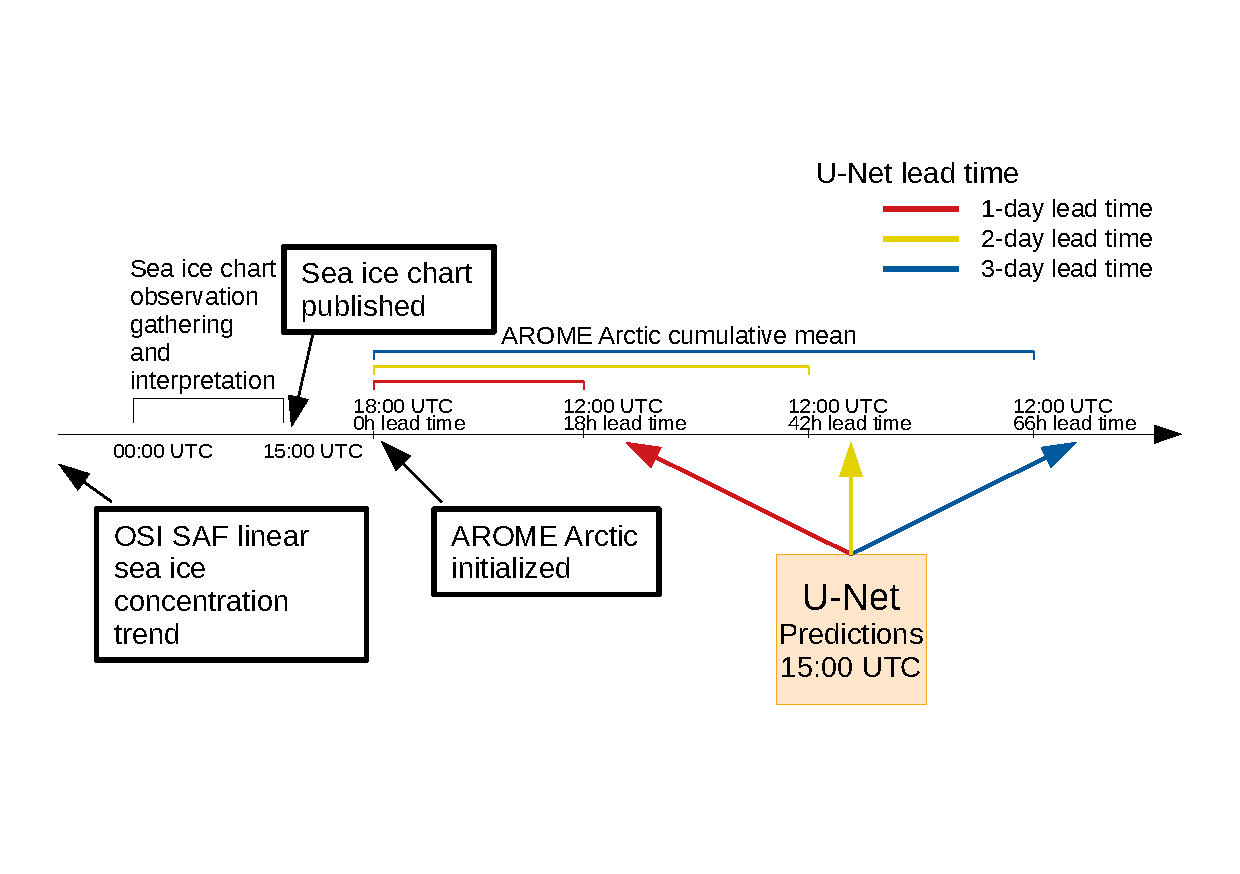
\includegraphics[width=\textwidth]{Predictor_schedule.pdf}
    \caption{\label{fig:pred_schedule}Overview of when the different predictors are published as well as forecast lead time and valid date for AROME Arctic and the Deep learning system. For clarity, a single bulletin date is shown, i.e. the shown predictors all goes into the Deep learning system initialized for a given date. The sea ice charts are published at 15:00 UTC, followed by AROME Arctic which is initialized at 18:00 UTC (available $\sim$20:30 UTC). The different colored AROME Arctic cumulative mean windows visualize which AROME Arctic lead-times are included when creating a sample for the Deep learning system for different Deep learning lead-times. The OSI SAF linear trend, which is computed from the day prior to the publication day of the predictor sea ice chart is included for completeness. U-Net is used as an abbreviation for the Deep learning system.}
\end{figure}

Figure \ref{fig:pred_schedule} also highlights that using AROME Arctic forecasts which was initialized earlier than 18:00 UTC to cover the 3 hour gap between the sea ice chart is published and AROME Arctic at 18:00 UTC is initialized would limit the ability to provide Deep learning predictions with a 3-day lead time. Hence the choice of using AROME Arctic initialized at 18:00 UTC is a compromise of achieving a 3-day lead time for the Deep learning system at the expense of missing atmospheric conditions the first three hours after the predictor sea ice chart is published.

All AROME Arctic data are stored as double precision floats (8 bytes), which when considering the target domain of $(1792 \times 1792)$ results in each field requiring $\approx 25.6 Mb$ of memory. Because predictors and model variables are stored in memory at the same time, predictor formulations which reduce the amount of memory reserved for each input variable has been explored. In the case of AROME Arctic data, instead of inputting each relevant timestep for each field as a stack of separate predictors, a cumulative mean along the temporal dimension between forecast initialization and 12:00 UTC at target valid-date is computed. Thus, the memory requirements for each AROME Arctic field is reduced while temporal changes is encoded into the variable as it supplies the network information about the mean state of the 10-meter winds and 2-meter temperature during the forecasted period. 

Studies such as \citet{Obite2020} have shown that artificial neural networks model multicollinear data better compared to traditional ordinary least squares regression, which indicates that feature engineering is less necessary for machine learning models. However the negative impacts of multicollinear predictors such as interdependance between variables and difficulties measuring the impact of a single variable still persist for deep learning methods \citep{Chan2022}. As such, providing AROME Arctic predictors as cumulative temporal mean fields intends to reduce the memory requirements of each predictor which enables greater batch sizes. Concurrently, the cumulative mean formulation may also aid to mitigate problems related to predictor multicollinearity.

The wind fields extracted from AROME Arctic are the u and v wind component at 10-meter height, i.e. the zonal and meridional wind components. However, the zonal and meridional wind components do not retain the same orientation throughout the region covered by the study area since the region is located at high latitudes. Hence the u and v components of the 10-meter winds are transformed to align with the x and y directions of the model domain. This ensures that the x and y wind fields are normal components with respect to each other at all locations due to the equidistant property of the grid, as well as providing all local neighborhoods considered in a convolutional layer with winds aligned in parallel.

\subsubsection{Targets}
\label{sec:data_targets}
The U-Net architecture adopted for this work performs classification, similarly to the U-Net outlined by \citet{Ronneberger2015}. Thus the sea ice concentration categories present in the sea ice charts \citep{Dinessen2020} will be used as ground truth labels when training the deep learning system. Furthermore, as the purpose of the model is to forecast the future state of sea ice concentration categories, the target sea ice chart will be one to three days after the sample creation date depending on the choice of forecast lead time. Otherwise, as the sea ice concentration targets are drawn from the same pool as predictor sea ice charts, the same preparation considerations are applied.

Motivated by the sea ice concentration distribution presented in Figure \ref{fig:2022-areadist-sic} along with limited fraction of the spatial domain covered by the MIZ ($0.15 \leq \text{sic} \leq 0.80$) as seen in the sea ice charts (e.g. figure \ref{fig:icechart}) and figure 2 in \citet{Strong2012}, each sea ice concentration category in the sea ice chart is defined as cumulative contours and predicted independently. In terms of the U-Net architecture, instead of having a singular output layer (turqoise arrow in figure \ref{fig:unet-overview}), the U-Net has individual output layers for each target sea ice concentration. Since each sea ice category represents a range of sea ice concentrations \citep{Dinessen2020}, each cumulative contour contains sea ice concentration categories equal to or greater than the lowermost category used to define the contour. This way, each cumulative contour represents a greater fraction of the domain than the individual classes, and predicting each contour separately is thought to be a more balanced prediction task than predicting all classes simultaneously following the original U-Net architecture \citep{Ronneberger2015}.

The mathematical definition of cumulative contours are given as follows. let $C \in \mathbb{R}^3$ be a set representing $(N > 2)$ contour elements with spatial indexes $i,j$ and elements $c_{i,j}^n$. Moreover, let $S \in \mathbb{R}^2$ represents a sea ice chart, with $s_{i,j}$ being the sea ice concentration values between 0 and 1. Then, let $k_n \in [0,1]$ be thresholds 

\begin{equation}
    \label{eq:cum_number}
    0 \leq k_1 < k_2 < \ldots < k_n \leq 1
\end{equation}

Hence, each cumulative contour is defined as

\begin{equation}
    \label{eq:cum_contour}
    c_{i,j}^n = \begin{cases}
        1 & \text{if } s_{i,j} \geq k_n \\
        0 & \text{if } s_{i,j} < k_n
    \end{cases}
\end{equation}

By adopting the scheme presented in Equation \ref{eq:cum_contour}, a more balanced representation of each contour is intended. Contrary to predicting each contour simultaneously, where the target dataset is skewed in disfavor of the MIZ contours, the cumulative contours reduce the classification task into multiple binary predictions where each contour is given a larger spatial distribution. Further details regarding technical implementation and how each predicted contour is reconstructed into a sea ice chart can be found in Section \ref{sec:implementation}.

\subsubsection{Preparing and loading data}
\label{sec:dataloader}
Sections \ref{sec:data_seaicecharts}, \ref{sec:data_trend}, \ref{sec:data_arome} and \ref{sec:data_targets} described how the data are preprocessed with respect to a common grid in addition to explaining how temporality is accounted for in the different datasets. The next step after the data are preprocessed is to store the data in predefined samples, as shown in Figure \ref{fig:data_pipeline}. For this work, a single sample is stored as an Hierarchial Data Format version 5 (.hdf5) file that make up the predictors and target for a given date at a given lead time. Hence, each lead time can be considered a separate dataset, as the composition of a sample differs based on the time difference between target and predictors. The choice of storing samples as individual files is made to limit the amount of memory needed to store all samples simultaneously in memory, although at the expected cost of increased I/O overhead. A single .hdf5 sample occupies 467 Megabytes of memory.

The main dataset used in this thesis covers the period between 2019 and 2022 due to the update to AROME Arctic in 2018 were an added snow on ice parameterization removed a significant temperature bias \citep{Batrak2019}. Regardless, datasets constructed from additional years will be inspected although specifically noted for clarity. Following common machine learning practices, the dataset is split into separate train, validation and test subsets. The data used for training and validating the deep learning model can be categorized in two distinct groups. The first group is the data known by the system, which is used during training to increase or validate model performance. Additional to the data used during training is external data, which is needed to validate the generalizability of the model. I.e., how well does the model perform with unknown data, which is assumed to be drawn from the same distribution as the data used during training. It is standard practice to arbitrarily split by a given fraction into the three datasets (training, validation, testing). However, due to the seasonal dependency seen in the current dataset, a naive split of the data could result in seasonally unbalanced datasets. As such, the data split is done manually such that each data subset covers at least a full year. Thus, no dataset is assumed to be seasonally skewed.

Currently the dataset is split such that 2022 is the test dataset, 2021 is the validation dataset and the years $\leq2020$ is the training dataset. See Table \ref{tab:data_subset_sizes} for a summary. However, it is noted that the above deterministic approach for splitting data deviates from common machine learning practices, where the data split is stochastic. A stochastic approach ensures especially that the test data is unknown to the developer as well as unseen by the model. Hence the latter approach associates less bias towards the data upon the model. Nevertheless an uneven seasonality is considered a greater detriment to model generalization than bias associated with a priori knowledge of the test dataset.

\begin{table}[]
    \caption{\label{tab:data_subset_sizes}Table showing the subset affiliation of each year, as well as the number of samples belonging to each year for all lead times. The dashed line is used to separate the core form the extended dataset, and represents the change in AROME Arctic following the implementation of \protect\citep{Batrak2019}.}
    \centering
    \setlength{\arrayrulewidth}{0.5mm}
    \renewcommand{\arraystretch}{1.3}
    \begin{tabular}{lllll}
    \hline
    year   & subset & 1 day lead time & 2 day lead time & 3 day lead time \\
    \hline
    2022 & test       & 196 & 147 & 142 \\
    2021 & validation & 198 & 147 & 142 \\
    2020 & train      & 198 & 146 & 142 \\
    2019 & train      & 192 & 143 & 144 \\
    \hdashline
    2018 & train      & 194 & 146 & 144 \\
    2017 & train      & 187 & 139 & 140 \\
    2016 & train      & 200 & 151 & 150 \\
    \hline         
    \end{tabular}
\end{table}

To increase the concurrency during training, a custom dataloader has been developed which reads data and prepares samples simultaneously as the model trains on previously loaded samples. The preparations performed by the dataloader is twofold. The dataloader first normalize the predictors according to the min-max normalization equation 

\begin{equation}
    x' = \frac{x - min_s(x)}{max_s(x) - min_s(x)}
\end{equation}

where $x$ is the predictor with $'$ denoting the normalized variant. Subscript $s$ refers to the subset minimum and maximum, implying the minimum and maximum of an entire data subset (train / validation / test). Each predictor is normalized according to a separate global minimum and maximum. Restricting the normalized data between $\left[0, 1\right]$ through min-max normalization ensures that the numerical predictors such as atmospheric data from AROME Arctic and the OSI SAF trend fall within the same value range as the categorical sea ice chart and land sea mask predictors. Min-max normalization is preferred for the current problem as it is invariant to the predictors being drawn from different distributions, e.g. the sea ice charts in Figure \ref{fig:2022-areadist-sic} resembles a heavy tailed distribution whereas 2-meter temperature from AROME Arctic would have a Gaussian distribution, since all predictors are scaled to the same range.

After normalization, the dataloader separates the target sea ice chart into individual binary contours constructed cumulatively as described previously in Section \ref{sec:data_targets}. During training, the dataloader also ensures that the samples are shuffled at the start of each epoch, which generalizes the optimizer (see e.g. Equation \ref{eq:msgd}) as the computed gradient of the loss is not biased towards the sample sequence.

\subsection{Model implementation}
\label{sec:implementation}
The purpose of this subsection is to describe the implemented deep learning architecture. Considerations taken with respect to the format of the input data will be explored, such as the decomposition of the target ice chart into cumulative contours explained in Section \ref{sec:data_targets}. Initial choices made, as well as integration of recent developments in deep learning based image processing will also be described.

\subsubsection{Overall structure of the network}
The developed model adopts the overall encoder-decoder structure of the U-Net architecture as described previously in Section \ref{sec:unet}. The model architecture can be decomposed into four main components, the input layer, encoder, decoder and output layers. Moreover, both the encoder and decoder consist of multiple convolutional blocks, which chain together a string of computations. The following sections will describe the technical details of each model component. The U-Net was developed using the machine learning framework Tensorflow v2.11 \citep{tensorflow2015-whitepaper} together with the Keras library \citep{chollet2015keras} using the Python v3.8.10 programming language. 

\subsubsection{Input layer}
The future state of sea ice concentration is predicted on lead times 1 - 3 days using the current ice chart, atmospheric predictors from AROME Arctic as well as the linear sea ice concentration trend derived from OSI SAF passive microwave observations (Section \ref{sec:dataloader}). These predictors creates a sample consisting of 7 channels. The spatial shape of each predictor has been set to $1792 \times 1792$ and covers parts of the European Arctic as shown in section (\ref{sec:roi}). The spatial size was set to be the even number 1792, as it is four times divisible by 4, thus allowing for four consecutive pooling operations of size $(4 \times 4)$ in the encoder \citep{Ronneberger2015} each reducing the domain by a factor of 4. 

Another reason for the reduced domain extent was to limit the amount of memory needed when loading data during training. The AROME Arctic domain has a spatial shape of $2370 \times 1845$ after being resampled onto a 1km grid. A reduced spatial shape also reduces the number of computations performed in the network at each layer, which speeds up training. The southern and eastern extent of the domain was trimmed due to considerations of the expected sea ice dynamics with the goal to avoid targeting likely sea ice concentration containing grid cells. First, there is no sea ice expected to occur at the southernmost grid cells. Second, the eastern part of the domain only experiences freezing during winter \citep{Serreze2019}.

\subsubsection{Encoder}
The encoder captures spatial features including temporal structures for the predictors with embedded temporality, which are used to capture the context of the scene \citep{Ronneberger2015}. The encoder is constructed by stacking a sequence of convolutional blocks with average pooling layers. Average pooling is similar to max pooling as it downsamples what is given as input, however instead of choosing the maximum value from a sliding filter the layer reduces what is seen by the filter to a mean value. Average pooling is described in Figure \ref{fig:avgpool}.

\begin{figure}
    \centering
    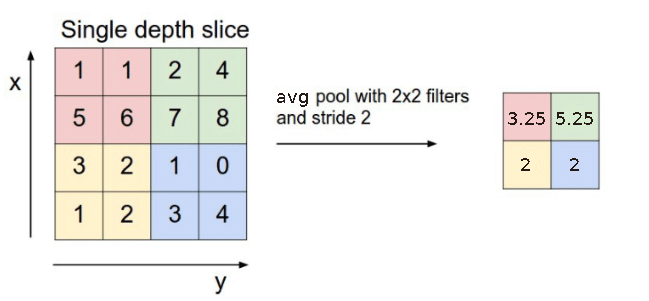
\includegraphics[width=0.9\textwidth]{The-AvgPool-operation.png}
    \caption{\label{fig:avgpool}The average pool operation for a $2 \times 2$ filter with a stride of 2. Figure modified from \protect\citet{MihaiDaniel2020}}
\end{figure}

Due to the large spatial extent of the input predictors, the average pooling layers are defined to have a $4 \times 4$ filter with a stride of 4. Hence, each pooling layer reduces the spatial size of the feature maps by a factor of 4, increasing the domain of influence captured by the receptive field of each pixel in the final feature map of the bottleneck.

\subsubsection{The convolutional block}
The convolutional block from \citet{Ronneberger2015} is adopted for this work, with both the $(3 \times 3)$ filter size and ReLU \citep{Nair2010} activation functions. To retain the spatial size of the input scene, each convolution is performed with zero-padding, which was omitted in \citet{Ronneberger2015} as it has the potential to create visual artefacts in the border region. Each convolutional block contains two convolutional layers with $2^{6 + n}$ number of output feature maps, where $n$ is the stage of the encoder starting from $n = 0$. Figure \ref{fig:unet-overview} shows how the number of feature maps follows the depth of the U-Net. The objective of the convolutional block is to detect features and construct feature maps from the incoming tensors, with each filter in the convolutional layers being sensitive only to a single pattern \citep{Fukushima1980}.

The current implementation of the convolutional block deviates from the original U-Net architecture as a normalization layer is added after each activation function to speed up and stabilize training \citep{Ioffe2015}. Although Batch Normalization has been commonly implemented in deep networks, works such as \citet{Wu2018} demonstrate that the technique exerts drawbacks for small batch size training. In \citet{Wu2018}, the drawbacks in batch normalization are attributed to the normalization statistics computed along the batch dimension of a feature map. Furthermore, \citet{Wu2018} presents an analogous technique for computing normalization statistics, albeit computed along the channel dimension which is divided into connected groups \citep{Wu2018}. The number of groups is set with a hyperparameter $G$. Figure \ref{fig:BNGN} shows the different normalization techniques in \citet{Ioffe2015} and \citet{Wu2018}.

\begin{figure}
    \centering
    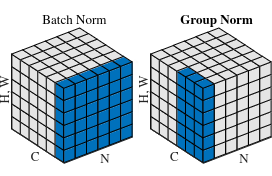
\includegraphics[width=0.35\textwidth]{BNandGN.png}
    \caption{\label{fig:BNGN}Schematic showing a feature map tensor of spatial shape (H,W) with N batches and C channels. The blue pixels are normalized by the same mean and variance. The group normalization hyperparameter $G = 2$. Figure modified from \protect\citet{Wu2018}}
\end{figure}

As increasing the batch size quickly saturates the available memory due to the high resolution predictors, group normalization is adapted for normalizing the feature maps. This follows the results in \citet{Wu2018} where group normalization was shown to reduce network error for small ($<8$) batch sizes. Following the recommendations by \citet{Wu2018}, the hyperparameter $G=32$. 

\subsubsection{Decoder}
The decoder restores the feature maps outputted by the encoder to image-resolution through the use of transposed convolutions \citep{Zeiler2010}. There are a similar amount of transposed convolutional layers as there are pooling layers, yet the number of convolutional blocks is reduced by one when compared to the encoder (see Figure \ref{fig:unet-overview}). The convolutional blocks in the decoder have the same structure as those used in the encoder. Each transposed convolution has a filter size and stride equal to the pooling factor, which has been set to 4. Moreover, the output space for each transposed convolution is $2^{5 - m + n_{\text{max}}}$ starting with $m = 0$ for the first transposed convolutional layer.

\subsubsection{Output layers}
\label{sec:architecture-output}
The feature maps at the final stage of the encoder is fed to the output component of the network. The output component is comprised of $C$ individual output layers (convolutional layer with $(1 \times 1)$ filter size, similarly sized as in \citet{Ronneberger2015}). However, the number of output channels of each output layer has been reduced to $1$, following the definition of cumulative target contours described in section (\ref{sec:data_targets}). With this described change to the network architecture, the computational graph following the decoder is changed such that the decoded signal is sent to $C$ different output layers (in Figure \ref{fig:unet-overview} this would be shown as $C$ turquoise arrows). Furthermore each output layer facilitates a binary classification task in which each pixel is predicted to belong in the cumulative contour associated with the layer. Finally, each prediction is activated pixel-wise with the sigmoid function (Equation \ref{eq:sigmoid}) which outputs a probability score $\left[0, 1\right]$ for belonging to the predicted contour. The output from the network has dimensions $(C, 1792, 1792, 1)$.

Given that each prediction is a spatially decreasing cumulative contour (see section \ref{sec:data_targets}), the predicted sea ice chart is constructed as a sum of the individual predictions along the first dimension of the model output. Here, it is assumed that the individual predictions adopt the cumulative property of the target cumulative contours. 

Initially, a more conventional architecture with a single output layer and multiple output categories \citep{Ronneberger2015} was attempted. Conversely, the model applies the softmax activation function (Equation \ref{eq:psoftmax}) to the outputs, which ensures that a single class is selected as most likely. However, due to unsatisfying results during the initial stages of development, further pursue of the architecture was dropped in favour of the above described model. An example prediction visualizing the problematic aspects of the model can be seen in Section \ref{sec:singleoutputmodel}. 

\subsubsection{Training environment}
\label{sec:train_env}
The model is trained on a GPU workstation with an Nvidia A100 80-Gb GPU available. The largest achievable batch-size in the environment was four. To both speed up training and reduce the memory footprint of the predictors, mixed precision training was utilized \citep{Micikevicius2017}. Mixed precision refers to storing the predictors as half-precision floats, whereas parameters in the model are stored as single-precision floats. Similarly to \citet{Ronneberger2015}, the model weights are HE-initialized \citep{He2015} since the ReLU activation function \citep{Nair2010} is used in the convolutional blocks.

The loss function implemented at each output layer is the pixelwise Binary Cross Entropy loss, which is an unweighted variation of the loss implemented in \citet{Ronneberger2015} (Equation \ref{eq:unet-loss}) for binary classification tasks. 

\begin{equation}
    \label{eq:loss}
    L = -\frac{1}{N}\sum_{n = 1}^N\sum_{p \in \mathbb{Z}^2}\left(y_p^n\log{(\hat{y}_p^n)} + \left(1 - y_p^n\right)\log{(1 - \hat{y}_p^n)}\right)
\end{equation}

where $N$ is the batch size, $y$ is the true label and $\hat{y}$ is the predicted probability by the model. Subscript $p$ refers to the pixels in $y$ and $\hat{y}$. As a consequence of the architecture described in Section \ref{sec:architecture-output}, the computed losses at each output layer exerts individual contributions to the convolutional layers after the split at the end of the decoder. Furthermore, at the end of the decoder, each loss contribution is reduced to a sum before further propagated through the network during backpropagation. The optimizer used is the ADAM optimizer \citep{Kingma2014}, and each model is trained for a maximum of 25 epochs.

Motivated by the bias-variance tradeoff described at the end of Section \ref{sec:training-loop}, a validation dataset is used to determine at which epoch the model achieves highest generalizability during training. Further motivated by the regularization effects offered by early stopping \citep{Graves2013}, while still allowing the network to converge further, a model checkpoint technique is deployed where the state of the model weights is stored every time the validational loss achieves a new minimum. As noted, the validation loss is monitored, which will be explored further in coming sections.


\subsection{Hyperparameter tuning and model selection}
\label{sec:model_development_results}
Throughout this section, the ice edge displacement metric is referred to frequently. If not otherwise stated, what is referred to is the IIEE of the $(> 10\%)$ contour normalized with respect to the climatological sea ice edge (section \ref{sec:osisafcdr}). Notations such as NIIEE refer to this metric. The details are described in the following section \ref{sec:clim_iceedge_compute}.

\subsubsection{Computing a climatological sea ice edge}
\label{sec:clim_iceedge_compute}
The IIEE \citep{Goessling2016} was derived in section \ref{sec:iiee} as an ice edge aware metric, which reports the average sea ice edge displacement error between two products when divided by the length of the sea ice edge \citep{Melsom2019}. Moreover, section \ref{sec:osisafcdr} presented the OSI SAF CDR as an independent observational product which will be utilized to derive a climatological sea ice edge which will serve as a normalization factor for the computed IIEE. When the IIEE was proposed by \citet{Goessling2016}, the metric was only assessed for coarse resolution, regional forecast data. Furthermore, it is unbeknownst to the author wether the IIEE or its normalized variation (NIIEE) has been used to assess the quality of high-resolution (1km) forecasts. What follows are considerations an experiments made to check the validity of utilizing the NIIEE for high-resolution forecasts.

The relationship between IIEE and a varying sea ice edge length is shown in figure \ref{fig:iiee_1km_10km}. The IIEE used in this figure was computed at 1km spatial resolution from the contour starting at 10\% sea ice concentration, with the resolution of the sea ice edge being varied. When computing the sea ice edge at 10km, both sea ice concentration fields were interpolated onto a 10km resolution grid using nearest neighbor interpolation. The correlation between the two NIIEE curves in figure \ref{fig:iiee_1km_10km} is 0.98.

\begin{figure}[h]
    \centering
    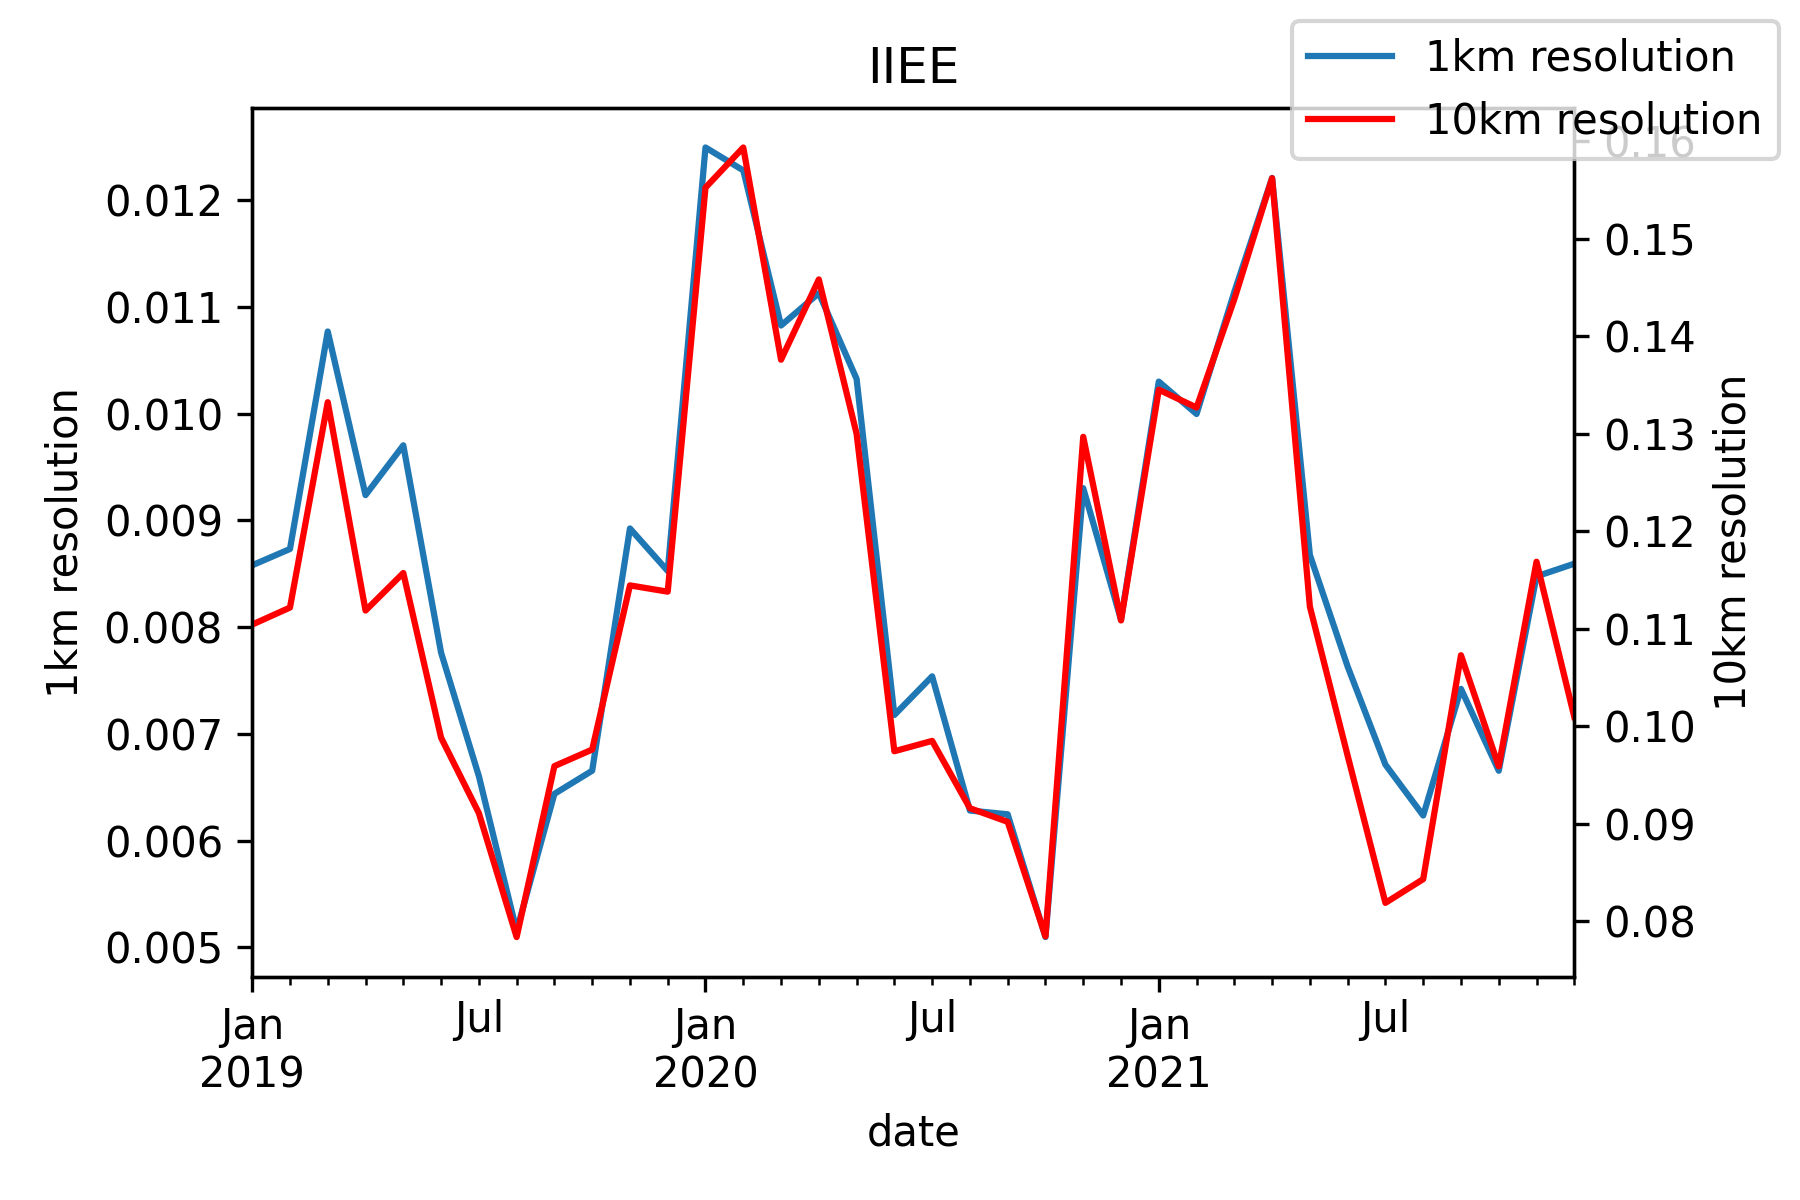
\includegraphics[width=1.\textwidth]{normalized_iiee}
    \caption{\label{fig:iiee_1km_10km}Integrated Ice Edge Error computed across three years (2019, 2020 and 2021) where the target is the sea ice charts and the forecast is persistence with a two day lead time. The IIEE was computed using a constant 1km spatial resolution for the sea ice concentration field, and a varying resolution for the sea ice edges. The ice edge length was computed as the mean sea ice edge length between the two products.}
\end{figure}

Moreover, the correlation between NIIEE computed from a 1km sea ice concentration field and a 1 km sea ice edge with the NIIEE computed from a 10km sea ice concentration field and 10 km sea ice edge is 0.98 as well. Finally, the mean difference between NIIEE from a 1km sea ice concentration field divided by a 10km sea ice edge and NIIEE from a 10km sea ice concentration field and a 10km sea ice edge is 0.1km.  

\subsubsection{Single output, multiple label model}
\label{sec:singleoutputmodel}
During early stages of model development, a version of the deep learning architecture with a single output layer and multiple target labels was developed. Figure (\ref{fig:singleoutmodel}) is an example prediction made with the described model. The intermediate categories very open drift ice $(10 - 30\%)$ and open drift ice $(40 - 60\%)$ are not resolved by the model, and persists for all samples (not shown). 

\begin{figure}
    \centering
    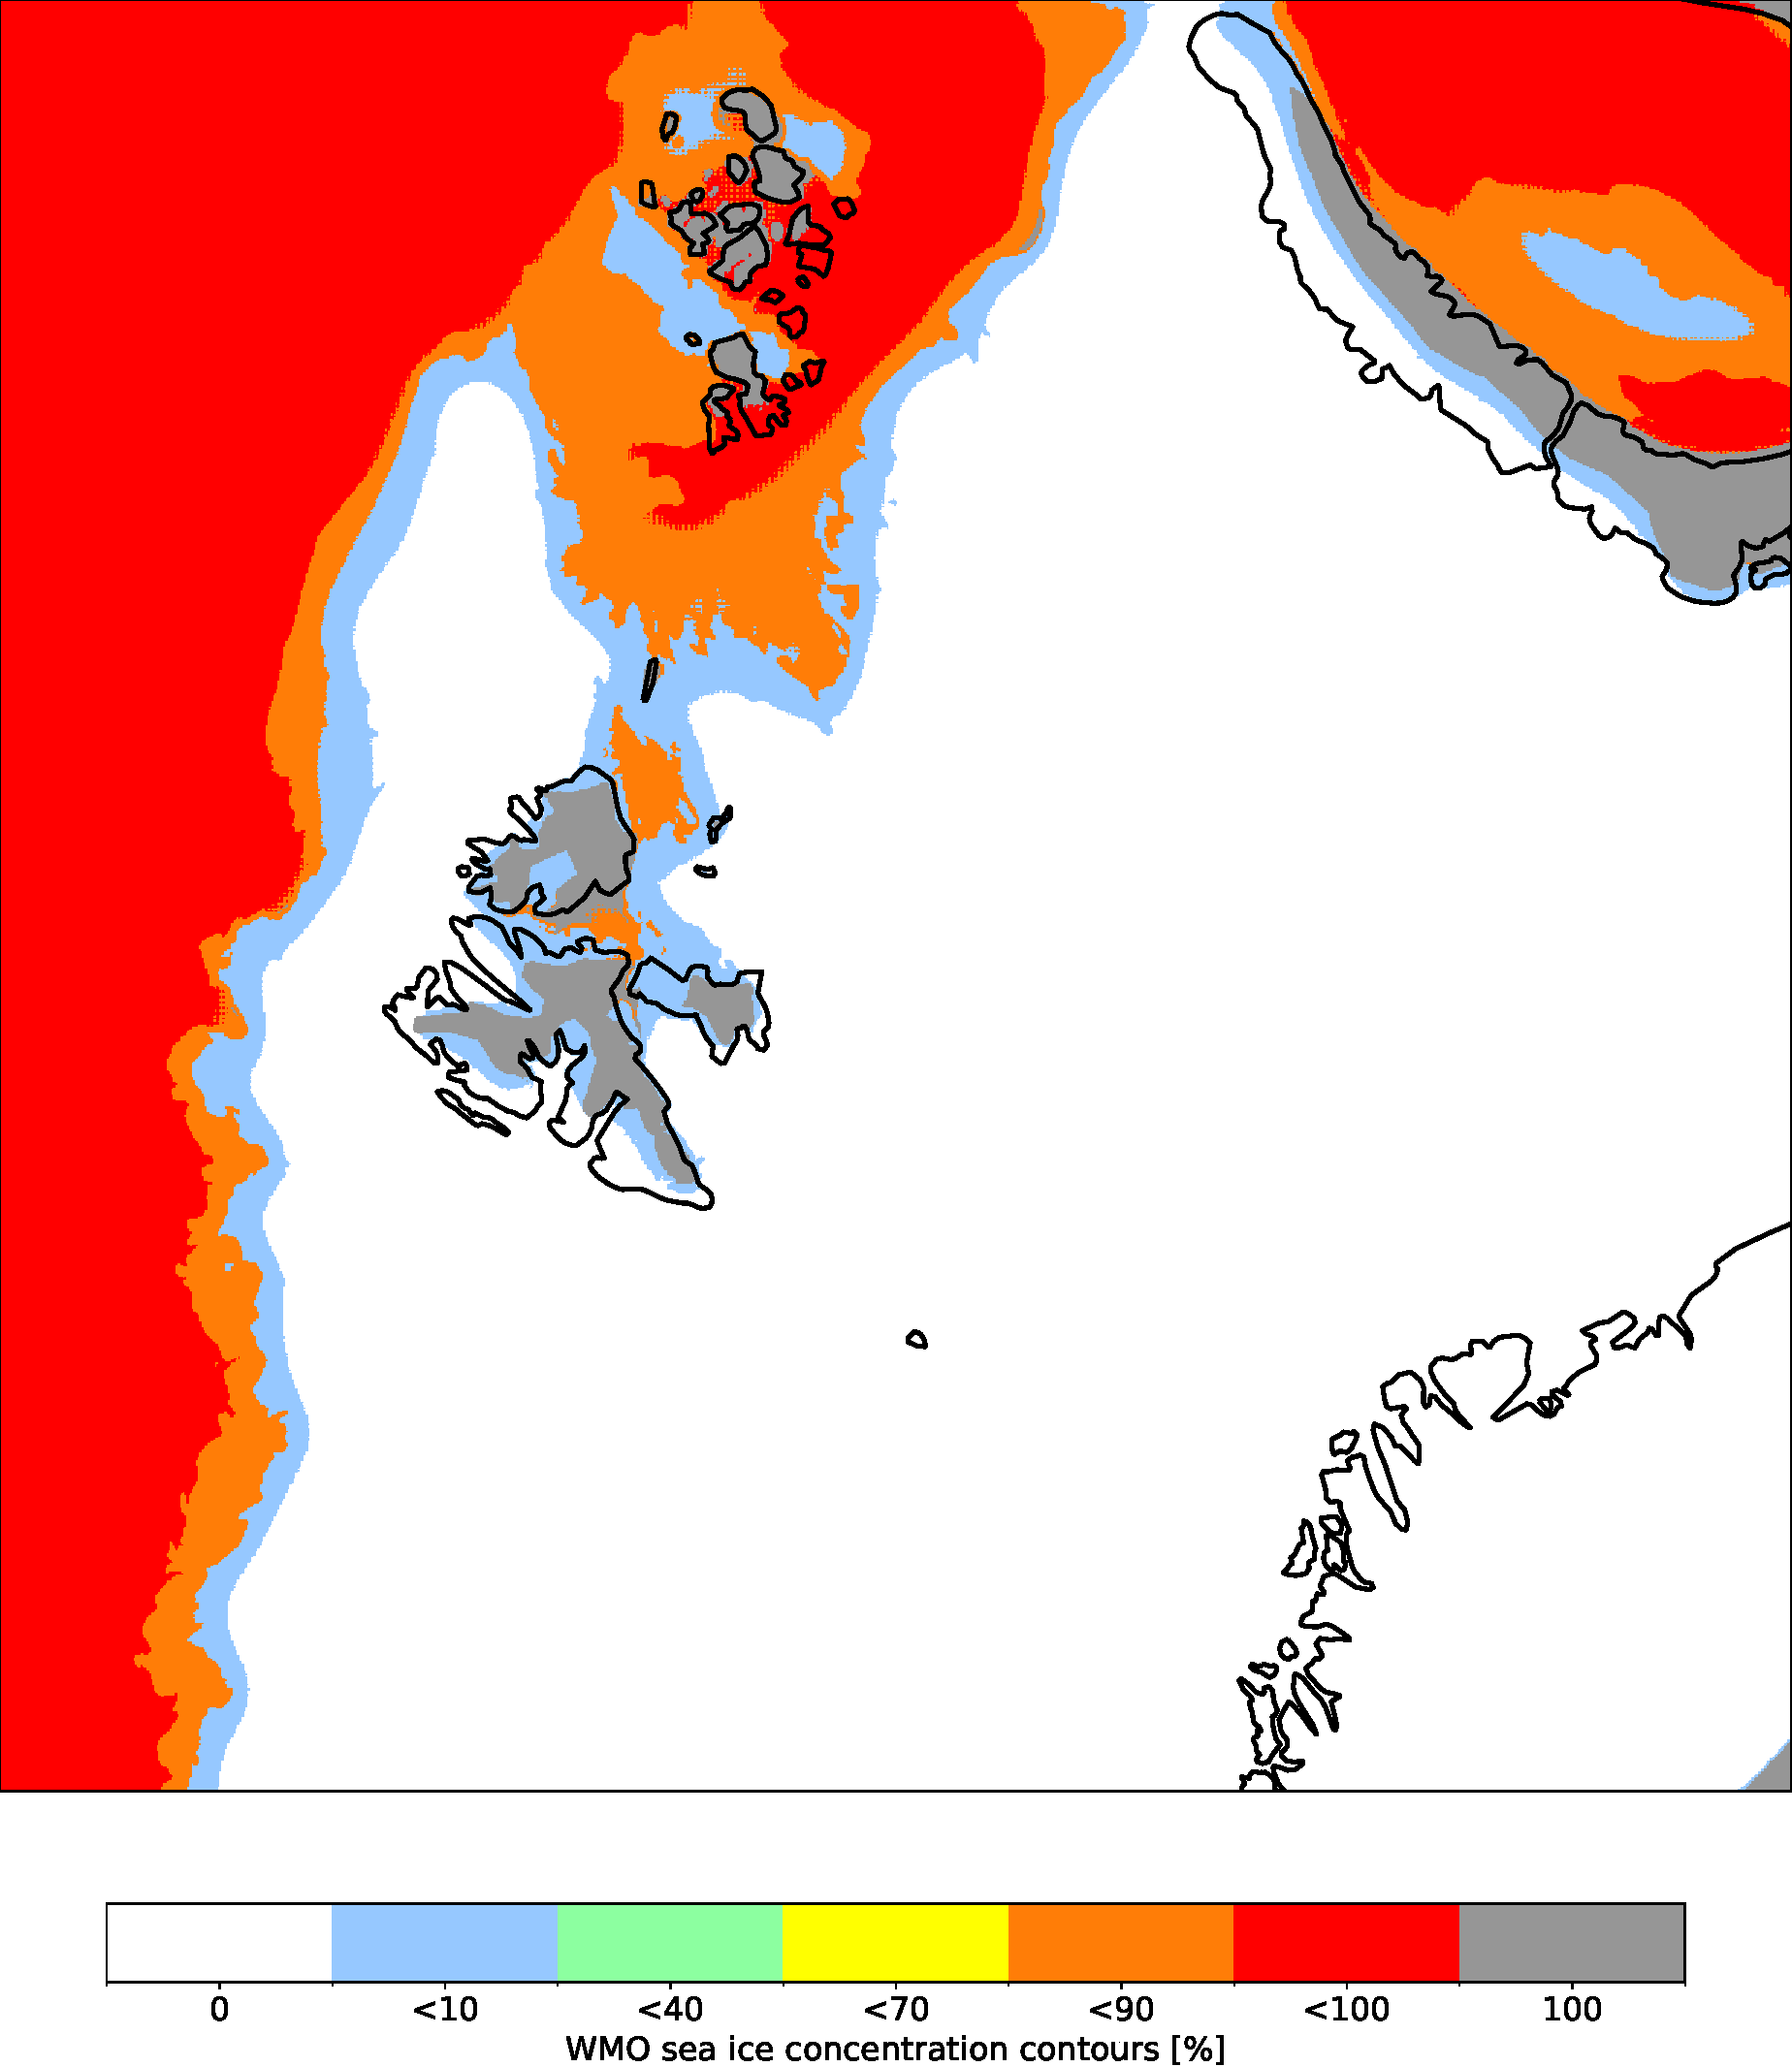
\includegraphics[width=.9\textwidth]{20210106}
    \caption{\label{fig:singleoutmodel}Prediction with a two day lead time, single output multiple labels U-Net 06 Jan 2021.}
\end{figure}

\subsubsection{General training performance}
Training the deep learning system for 25 epochs takes $\sim 3\text{h}30\text{min}$ on the GPU workstation, although the training time have varied positively and negatively following driver updates and other non-transparent backend operations. Iterating through the training data takes $\sim 6$ minutes, and the validation data $\sim 8$ minutes for a single epoch. Memory usage varies between $\sim19.4$ and $\sim55$ gb, and scales with the depth of the U-Net. With a pre-trained model, performing a single prediction on a workstation CPU (AMD EPYC 7282 16-Core) takes $\sim 6$ seconds, while on a laptop CPU (Intel(R) Core(TM) i7-8565U 8-Core) takes $\sim 30$ seconds.

To determine the optimal learning rate and U-Net depth, a grid search was conducted across variations of the aforementioned variables. The result is shown in figure \ref{fig:gs}. It can be seen from the figure that the validation loss increases with U-Net depth. At the same time, the validation loss also increases when the learning rate deviates from $0.001$.

\begin{figure}
    \centering
    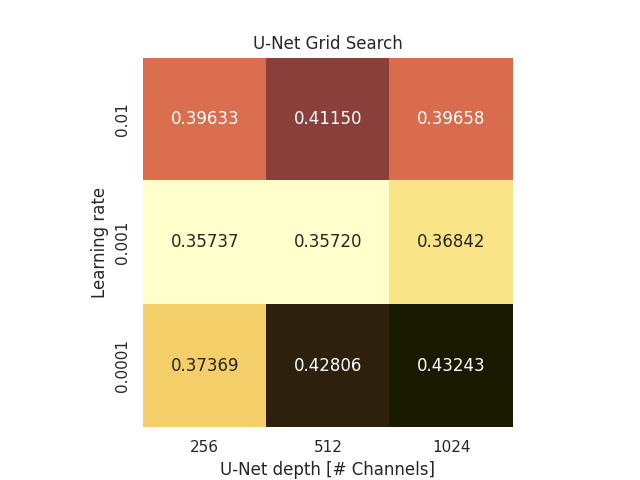
\includegraphics[width=.8\textwidth]{grid_search}
    \caption{\label{fig:gs}Grid search performed over variations of the learning rate as well as an increasing U-Net depth (represented by the number of feature maps at the at the final convolutional block). Each cell contains the minimum obtained validation loss for its respective combination.}
\end{figure}

Training curves for the model in figure \ref{fig:gs} which achieved a loss of 0.35737 ($\text{lr} = 0.001$, $\text{U-Net depth} = 256$) are shown in figure \ref{fig:loss_curve_from_gs}. The figure plots both the training and validation loss, as well as a third curve which keeps track of the current minimum validation loss. The lowest validational loss is achieved at epoch 17. 

\begin{figure}
    \centering
    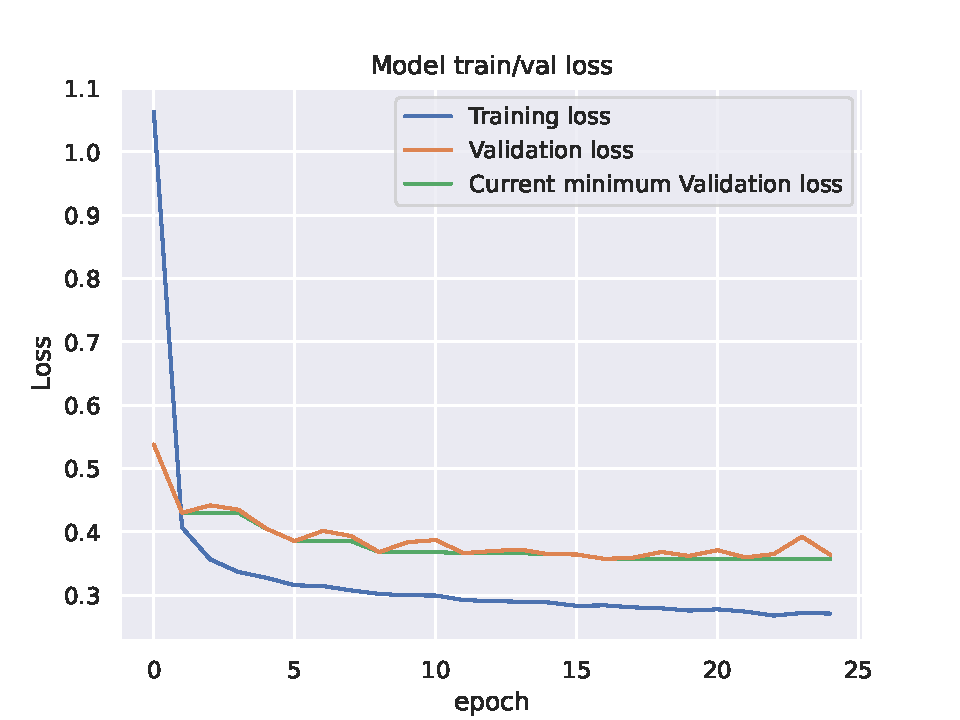
\includegraphics[width=\textwidth]{loss_curve_best_model_gs}
    \caption{\label{fig:loss_curve_from_gs}Training and validation loss from the middle leftmost model in Figure (\ref{fig:gs}) (lr = 0.001, depth = 256). The current minimum validation loss is also displayed.}
\end{figure}

Figure \ref{fig:256_1024_compare} shows the impact that model depth has on the predictions. Both models are trained on the same data, and the best model for both training procedures is selected according to section \ref{sec:train_env}. Both models resolve the scene comparatively, with mean annual statistics of ice edge displacement error being 28.2 km for the model in figure \ref{fig:256_1024_compare}a and 30.7 km for the model in figure \ref{fig:256_1024_compare}b. The total number of trainable parameters in the 256 architecture is $\sim 2.4$ million, where $\sim 1.15$ million are located in the encoder and $\sim 1.25$ million in the decoder. The rightmost model in figure \ref{fig:256_1024_compare}, which has a depth of 1024 filters, contain $\sim 16$ times more parameters than the model with a depth of 256 filters, with a total of $\sim39 $ million parameters. Decomposing the total number of parameters into encoder and decoder results in $\sim 19$ million parameters in the encoder and $\sim 20$ million parameters in the decoder. For reference, the 512 depth model contain $\sim 9.8$ million parameters. The receptive field of the bottleneck (final feature map in the encoder) for both models is calculated using equation \ref{eq:receptivefield}. The model with a depth of 256 has an encoder with a theoretical receptive field of 145 pixels in each spatial dimension, whereas the model with a depth of 1024 has an encoder with a theoretical receptive field of 2385 pixels in each direction. For the second model, a receptive field of 2385 results in the entire input scene being used as context for each pixel in the final encoder feature map. Note that the theoretical receptive field is invariant to the input shape.

\begin{figure}
    \centering
    \begin{subfigure}[t]{.03\textwidth}
        a)
    \end{subfigure}
    \begin{subfigure}[t]{0.455\textwidth}
        \centering
        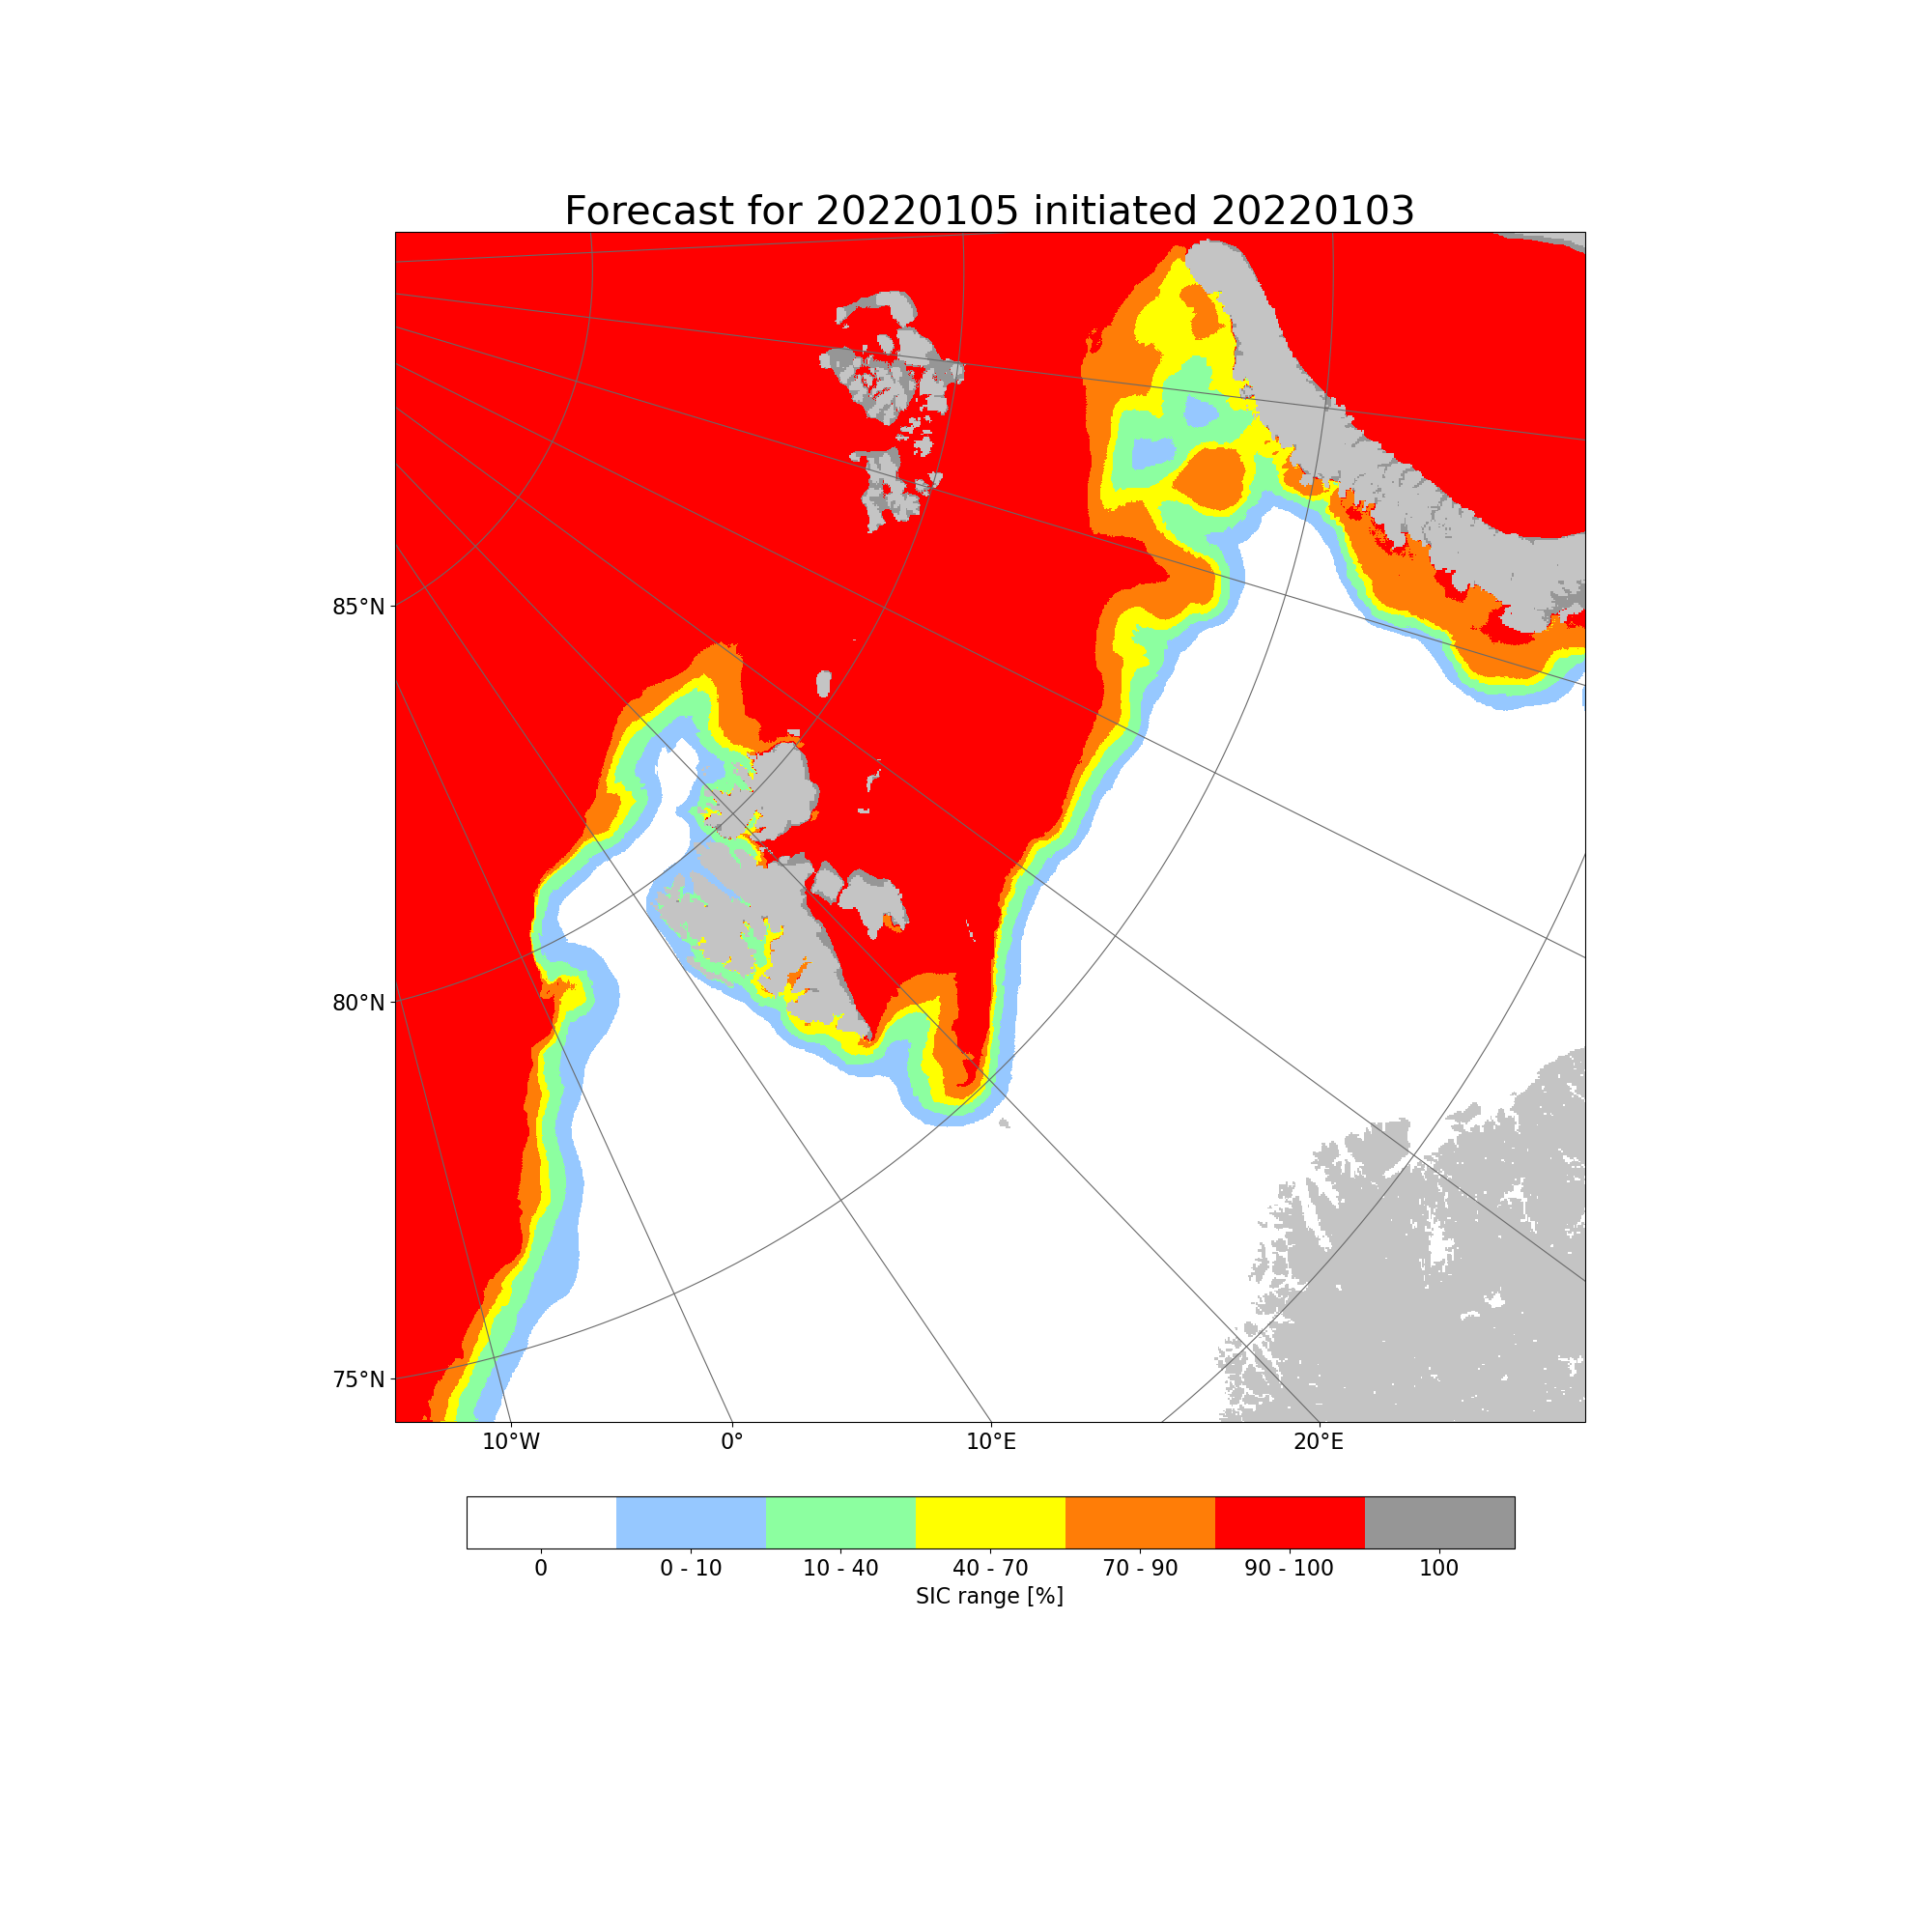
\includegraphics[width=\textwidth, valign=t]{unet_256_jan}
    \end{subfigure}\hfill
    \begin{subfigure}[t]{.03\textwidth}
        b)
    \end{subfigure}
    \begin{subfigure}[t]{0.455\textwidth}
        \centering
        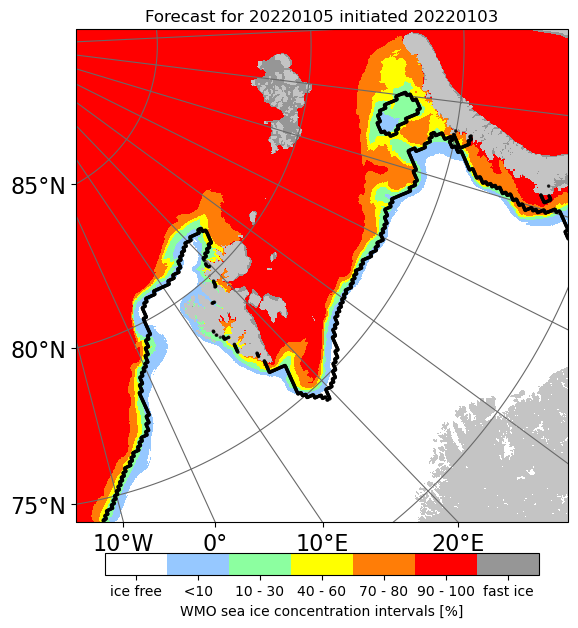
\includegraphics[width=\textwidth, valign=t]{unet_1024_jan}
    \end{subfigure}
    \caption{Prediction of 05 Jan 2022 with two different model architectures with a 2 day lead time. The model in the leftmost figure has lr = 0.001 and depth 256, contains $\sim 2.4$ million parameters, and achieves a mean annual ice edge displacement ($>10\%$ contour) of 28.2 km. The model in the rightmost figure has lr = 0.001 and a depth 0f 1024, contains $\sim 39$ million parameters, and achieves a mean annual ice edge displacement of 30.7 km. The black line is the 15\% sea ice edge computed from OSI SAF SSMIS.}
    \label{fig:256_1024_compare}
\end{figure}

A full year of forecasts, where each month is represented by the first prediction made that month using a 2 day lead time model and 256 architecture is shown in Figure \ref{fig:timeseries}. Figure \ref{fig:timeseries} also shows the sea ice edge computed from OSI SAF SSMIS observations at 10km spatial resolution. The figure is intended as an example of the predictive capabilities of the model across the entire test dataset. 

\begin{figure}
    \centering
    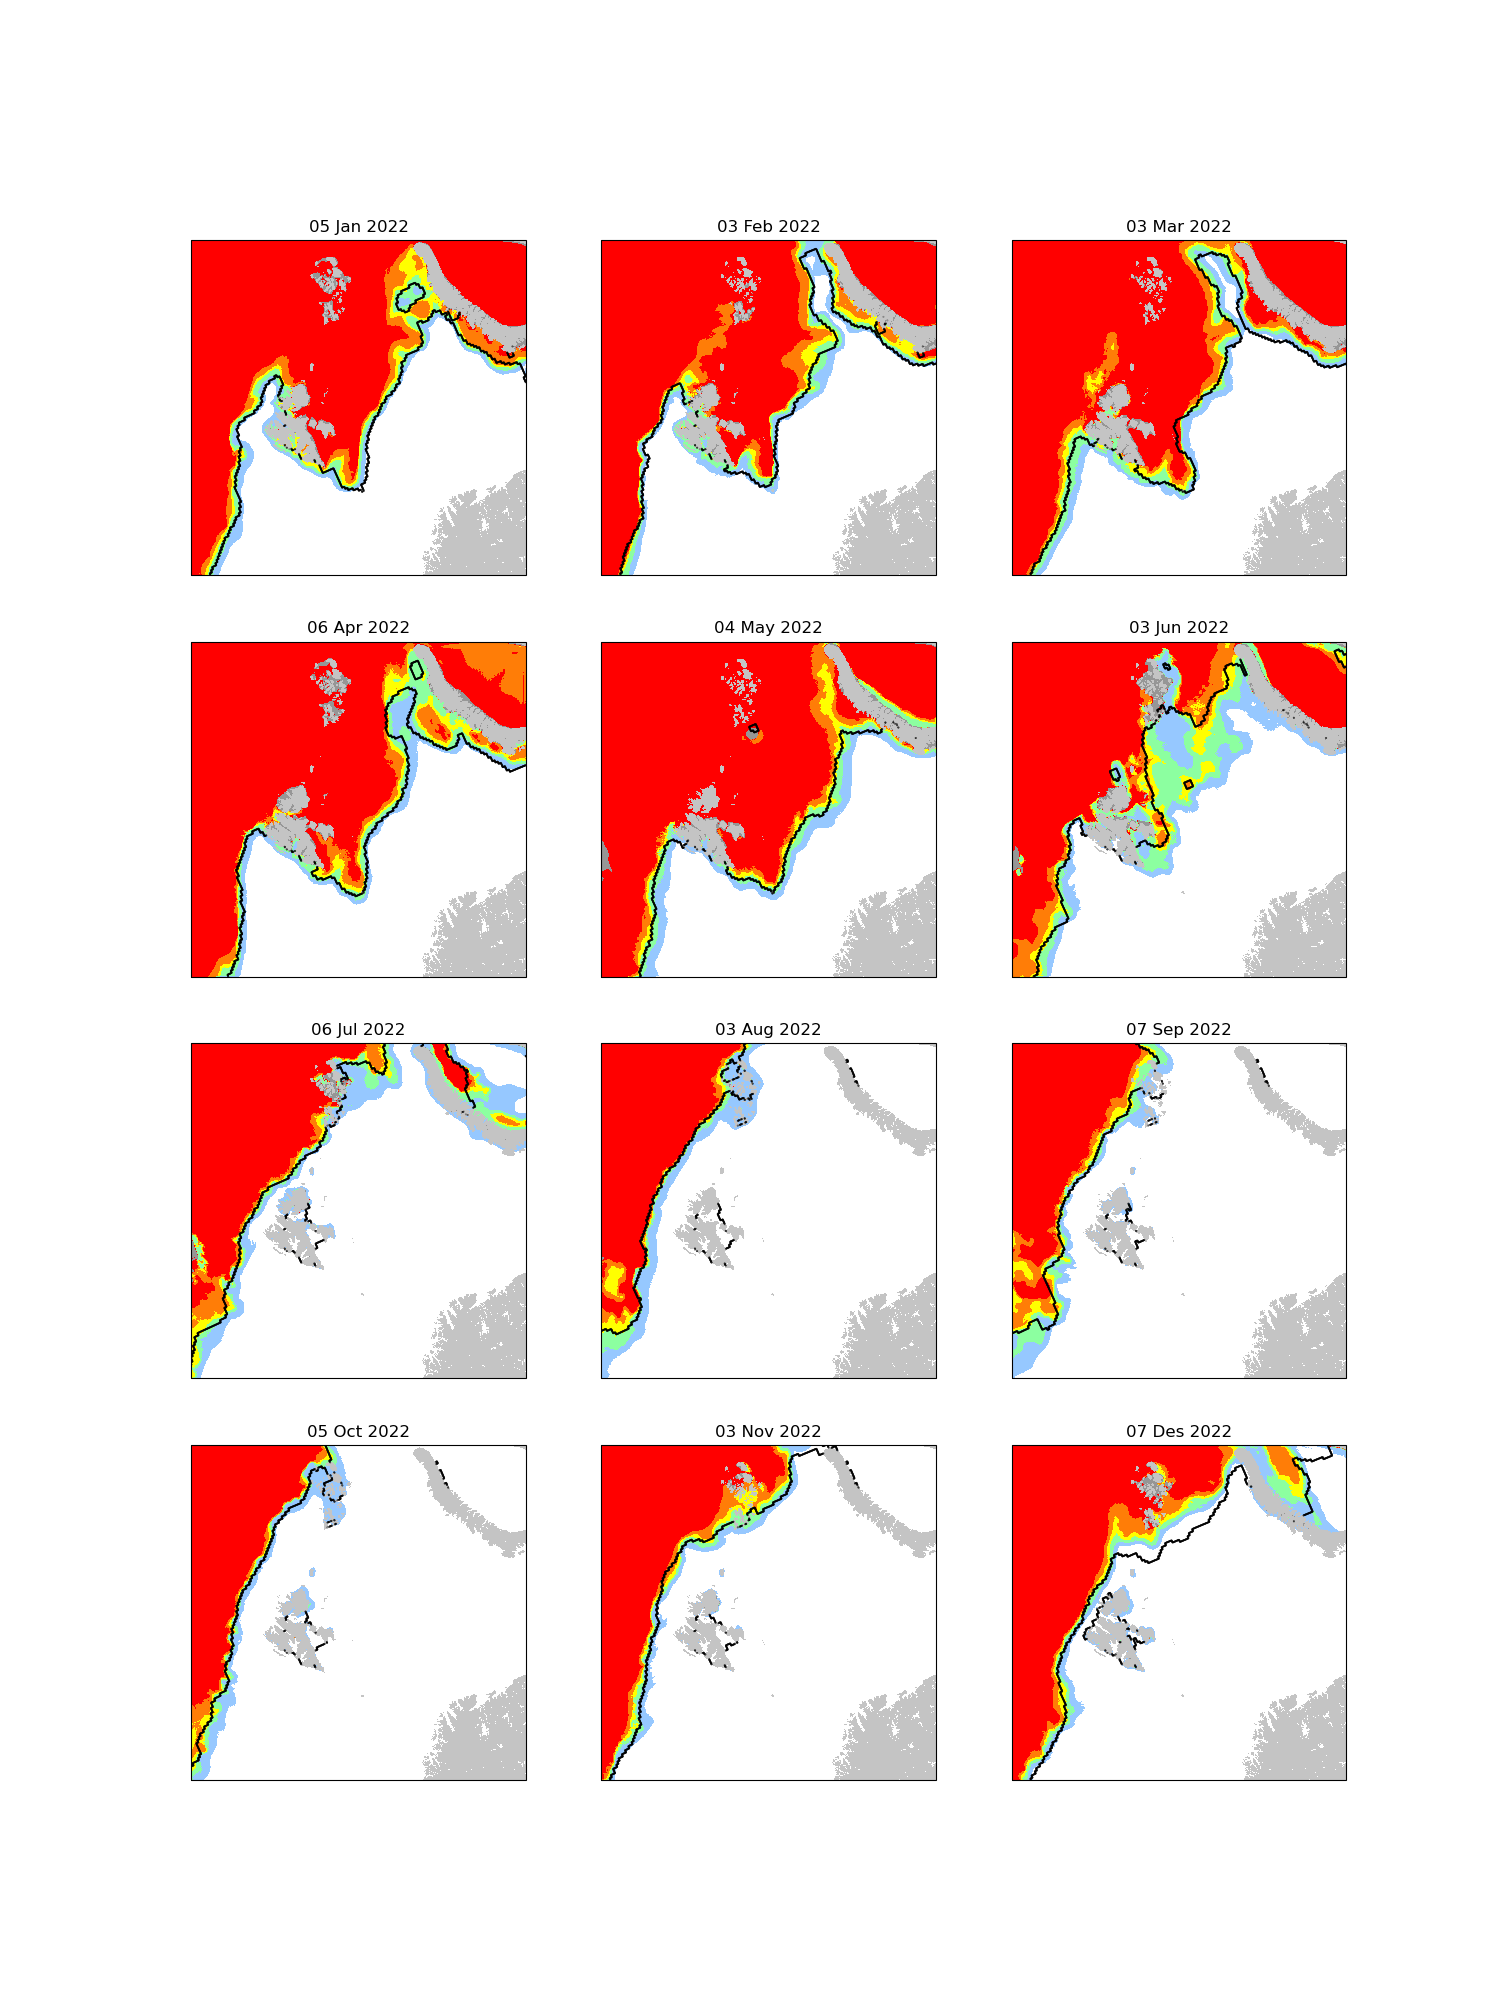
\includegraphics[width=.855\textwidth]{Forecast_time_series}
    \caption{\label{fig:timeseries}Prediction with a 2 day lead time given the first available ice chart each month of 2022. The black line is the 15\% ice edge computed from OSI SAF SSMIS. The figure exemplifies the predicitve capabilities of the model. Subplots for each month exemplifies seasonal variability of the model.}
\end{figure}

The effect of training across varying lead time is shown in Figure \ref{fig:lead_times}. From Figure \ref{fig:lead_times}a, it can be seen that both persistence and the deep learning forecast increase their mean annual NIIEE with increasing lead times. It can also be seen that persistence achieves a higher mean annual NIIEE than the deep learning model for all lead times. Figure \ref{fig:lead_times}b shows that the forecast improvement increases with the lead time, which follows the divergence between the deep learning and persistence NIIEE curves in Figure \ref{fig:lead_times}a. Note that it is expected for both persistence and the Deep learning model to lose skill with increasing lead time.

\begin{figure}
    \centering
    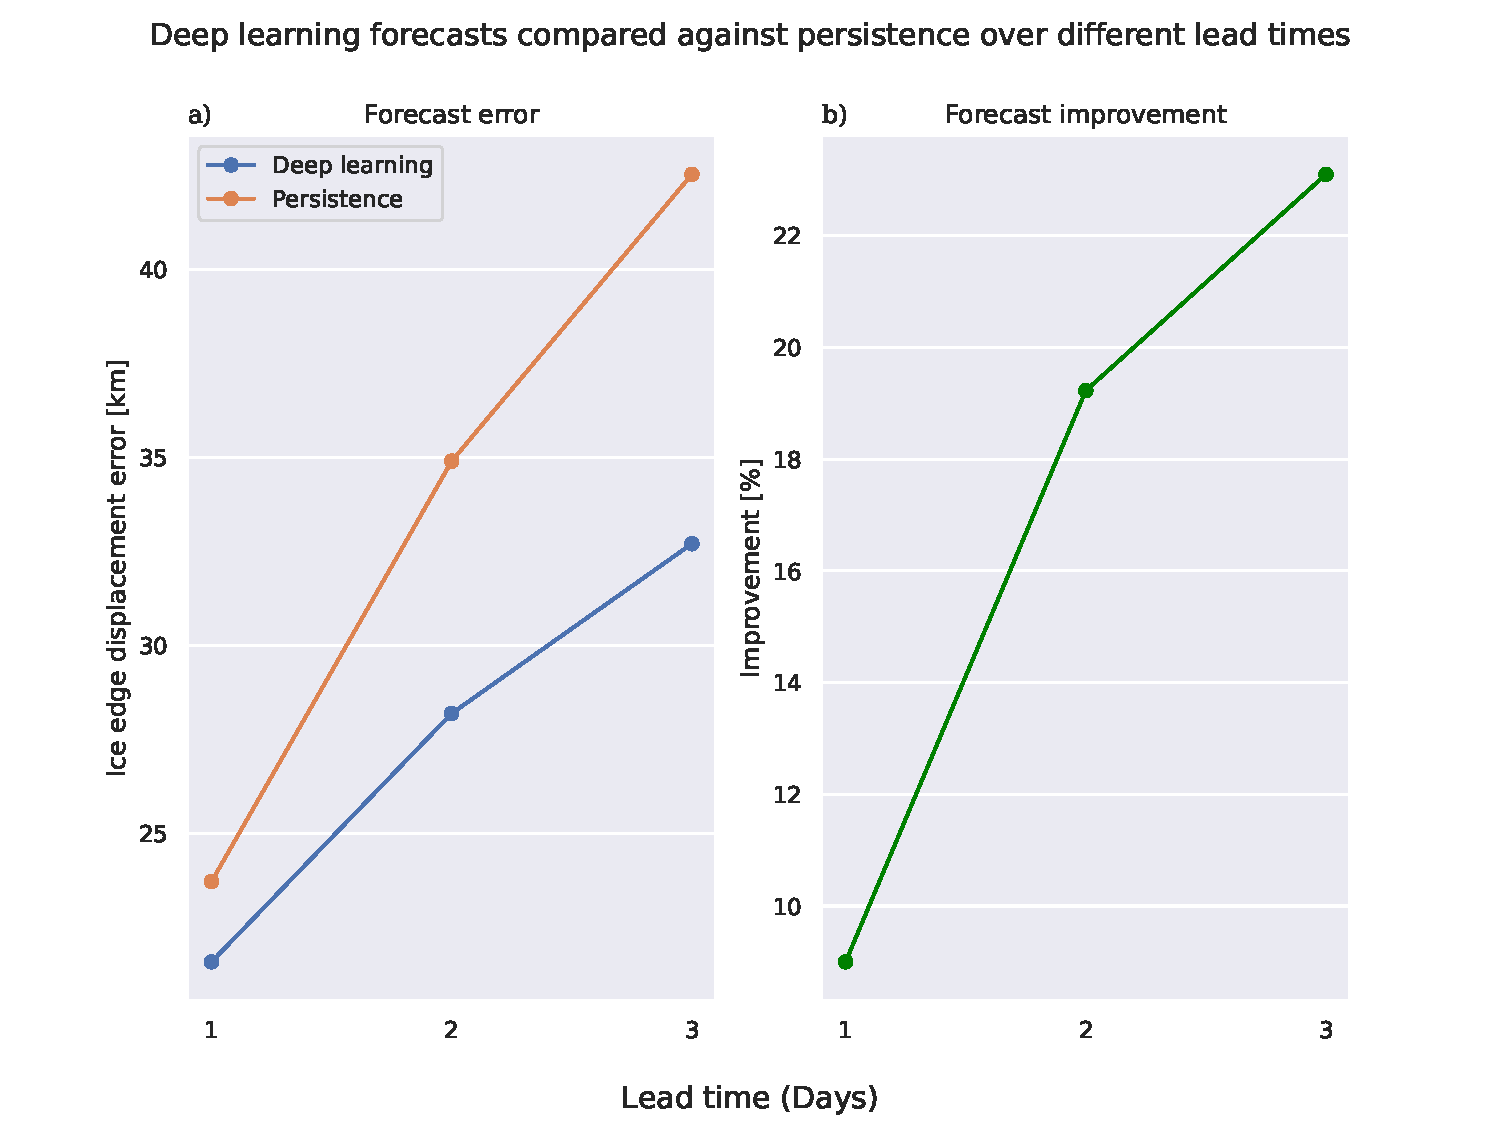
\includegraphics[width=\textwidth]{lead_times.pdf}
    \caption{\label{fig:lead_times}Comparing the effect of training the deep learning system against varying target lead time. The ice edge displacement reported in subfigure a) is the normalized IIEE with regards to the $(> 10\%)$ contour. The improvement compared to persistence in subfigure b) is computed in favour of the deep learning forecast.}
\end{figure}

An inspection on the effect of appending additional years to the core (2019 and 2020) training data is summarized in figure \ref{fig:append_years}. Both validation loss and NIIEE is shown in figure \ref{fig:append_years}. The model trained with a training dataset starting in 2016 and including all years up until including 2020 has higher validation loss (2021) and NIIEE (2022) than the other models in figure \ref{fig:append_years}. The model trained with the period 2017-2020 achieves the lowest score for both monitored metrics.

\begin{figure}
    \centering
    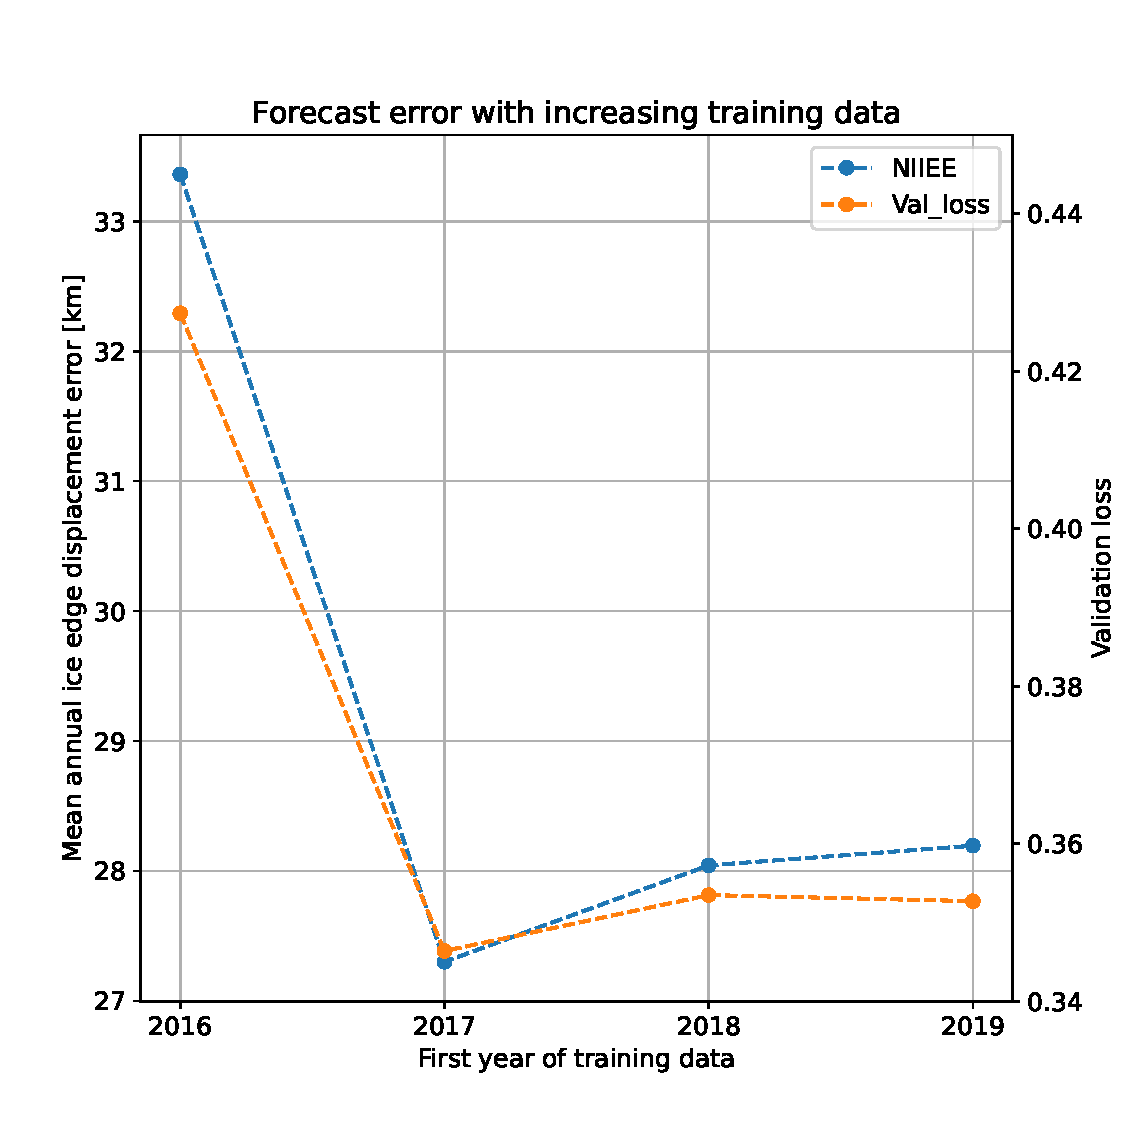
\includegraphics[width=.9\textwidth]{years_start.pdf}
    \caption{\label{fig:append_years}The lines visualize the relationship between start year for the training data (upper bound is always 2020) with the ice edge displacement error for the $(> 10\%)$ contour and validation loss.}
\end{figure}

An inspection of the interannual variability of the NIIEE and Sea Ice Extent of persistence with regards to a two day lead time for the years covered by the full extent of the training data (2016 to 2022) is shown in figure \ref{fig:NIIEE-and-SIE}. The sea ice extent shown in the topmost figure (a) in figure \ref{fig:NIIEE-and-SIE} is computed as the sum of all grid cell areas with category equal to or higher than the targeted contour. No discernable trend across the years can be seen in either (a) or (b) in figure \ref{fig:NIIEE-and-SIE} 

\begin{figure}
    \centering
    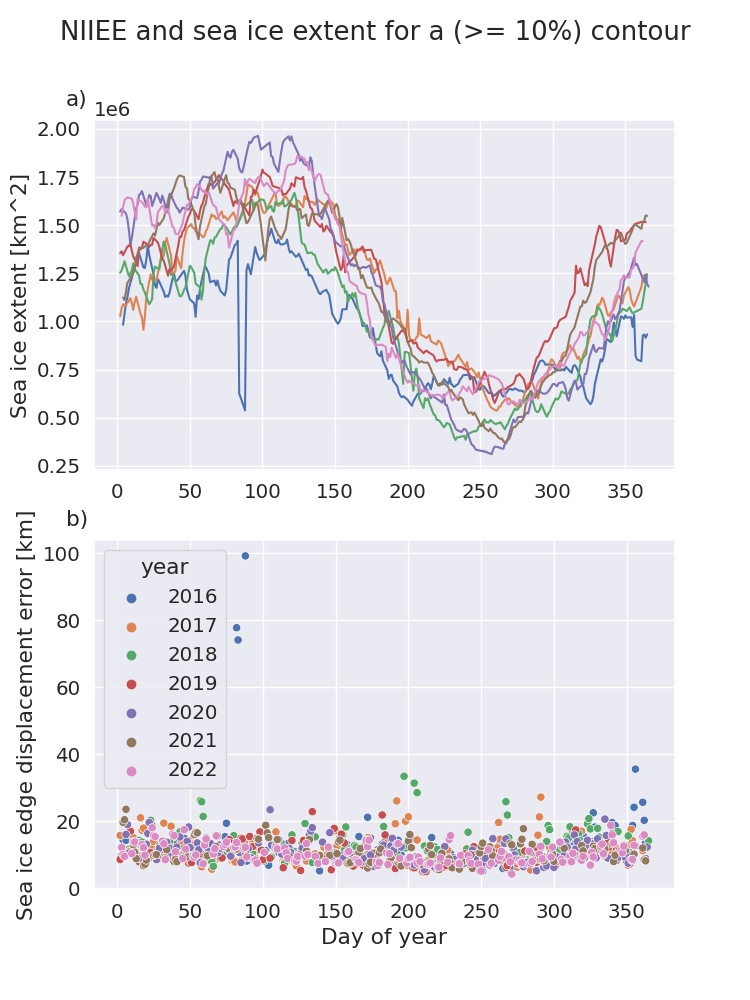
\includegraphics[width=.8\textwidth]{Persistence_NIIEE_SIE}
    \caption{\label{fig:NIIEE-and-SIE}Interannual variability of sea ice extent for the sea ice charts (a) and NIIEE (b) against persistence persistence for a two day lead time. The three outlier data-points from 2016 is associated with three dates (24/03, 25/03 and 28/03) where the sea ice charts were erroneously incomplete.}
\end{figure}

The impact of non-linear activation functions was assessed by training a model were the activation functions were replaced with a linear mapping. The mean annual NIIEE on the test set was 41.35 km, which is 13.15km more than the benchmark model with a mean annual NIIEE of 28.20 km. A qualitative prediction made with the model can be seen in figure \ref{fig:linear_model}. Inspecting figure \ref{fig:linear_model} reveals visual artefacts produced by the linear model, not seen in comparable predictions from non linear models. E.g. the sea ice contours east and west of Novaya Semlya exerts a prominent checkerboard-like pattern, which is repeated throughout the scene. Figure \ref{fig:linear_model} exemplifies that non-linear activation functions add skill to the Deep learning forecasts, beyond what is achievable by a linear model.

\begin{figure}
    \centering
    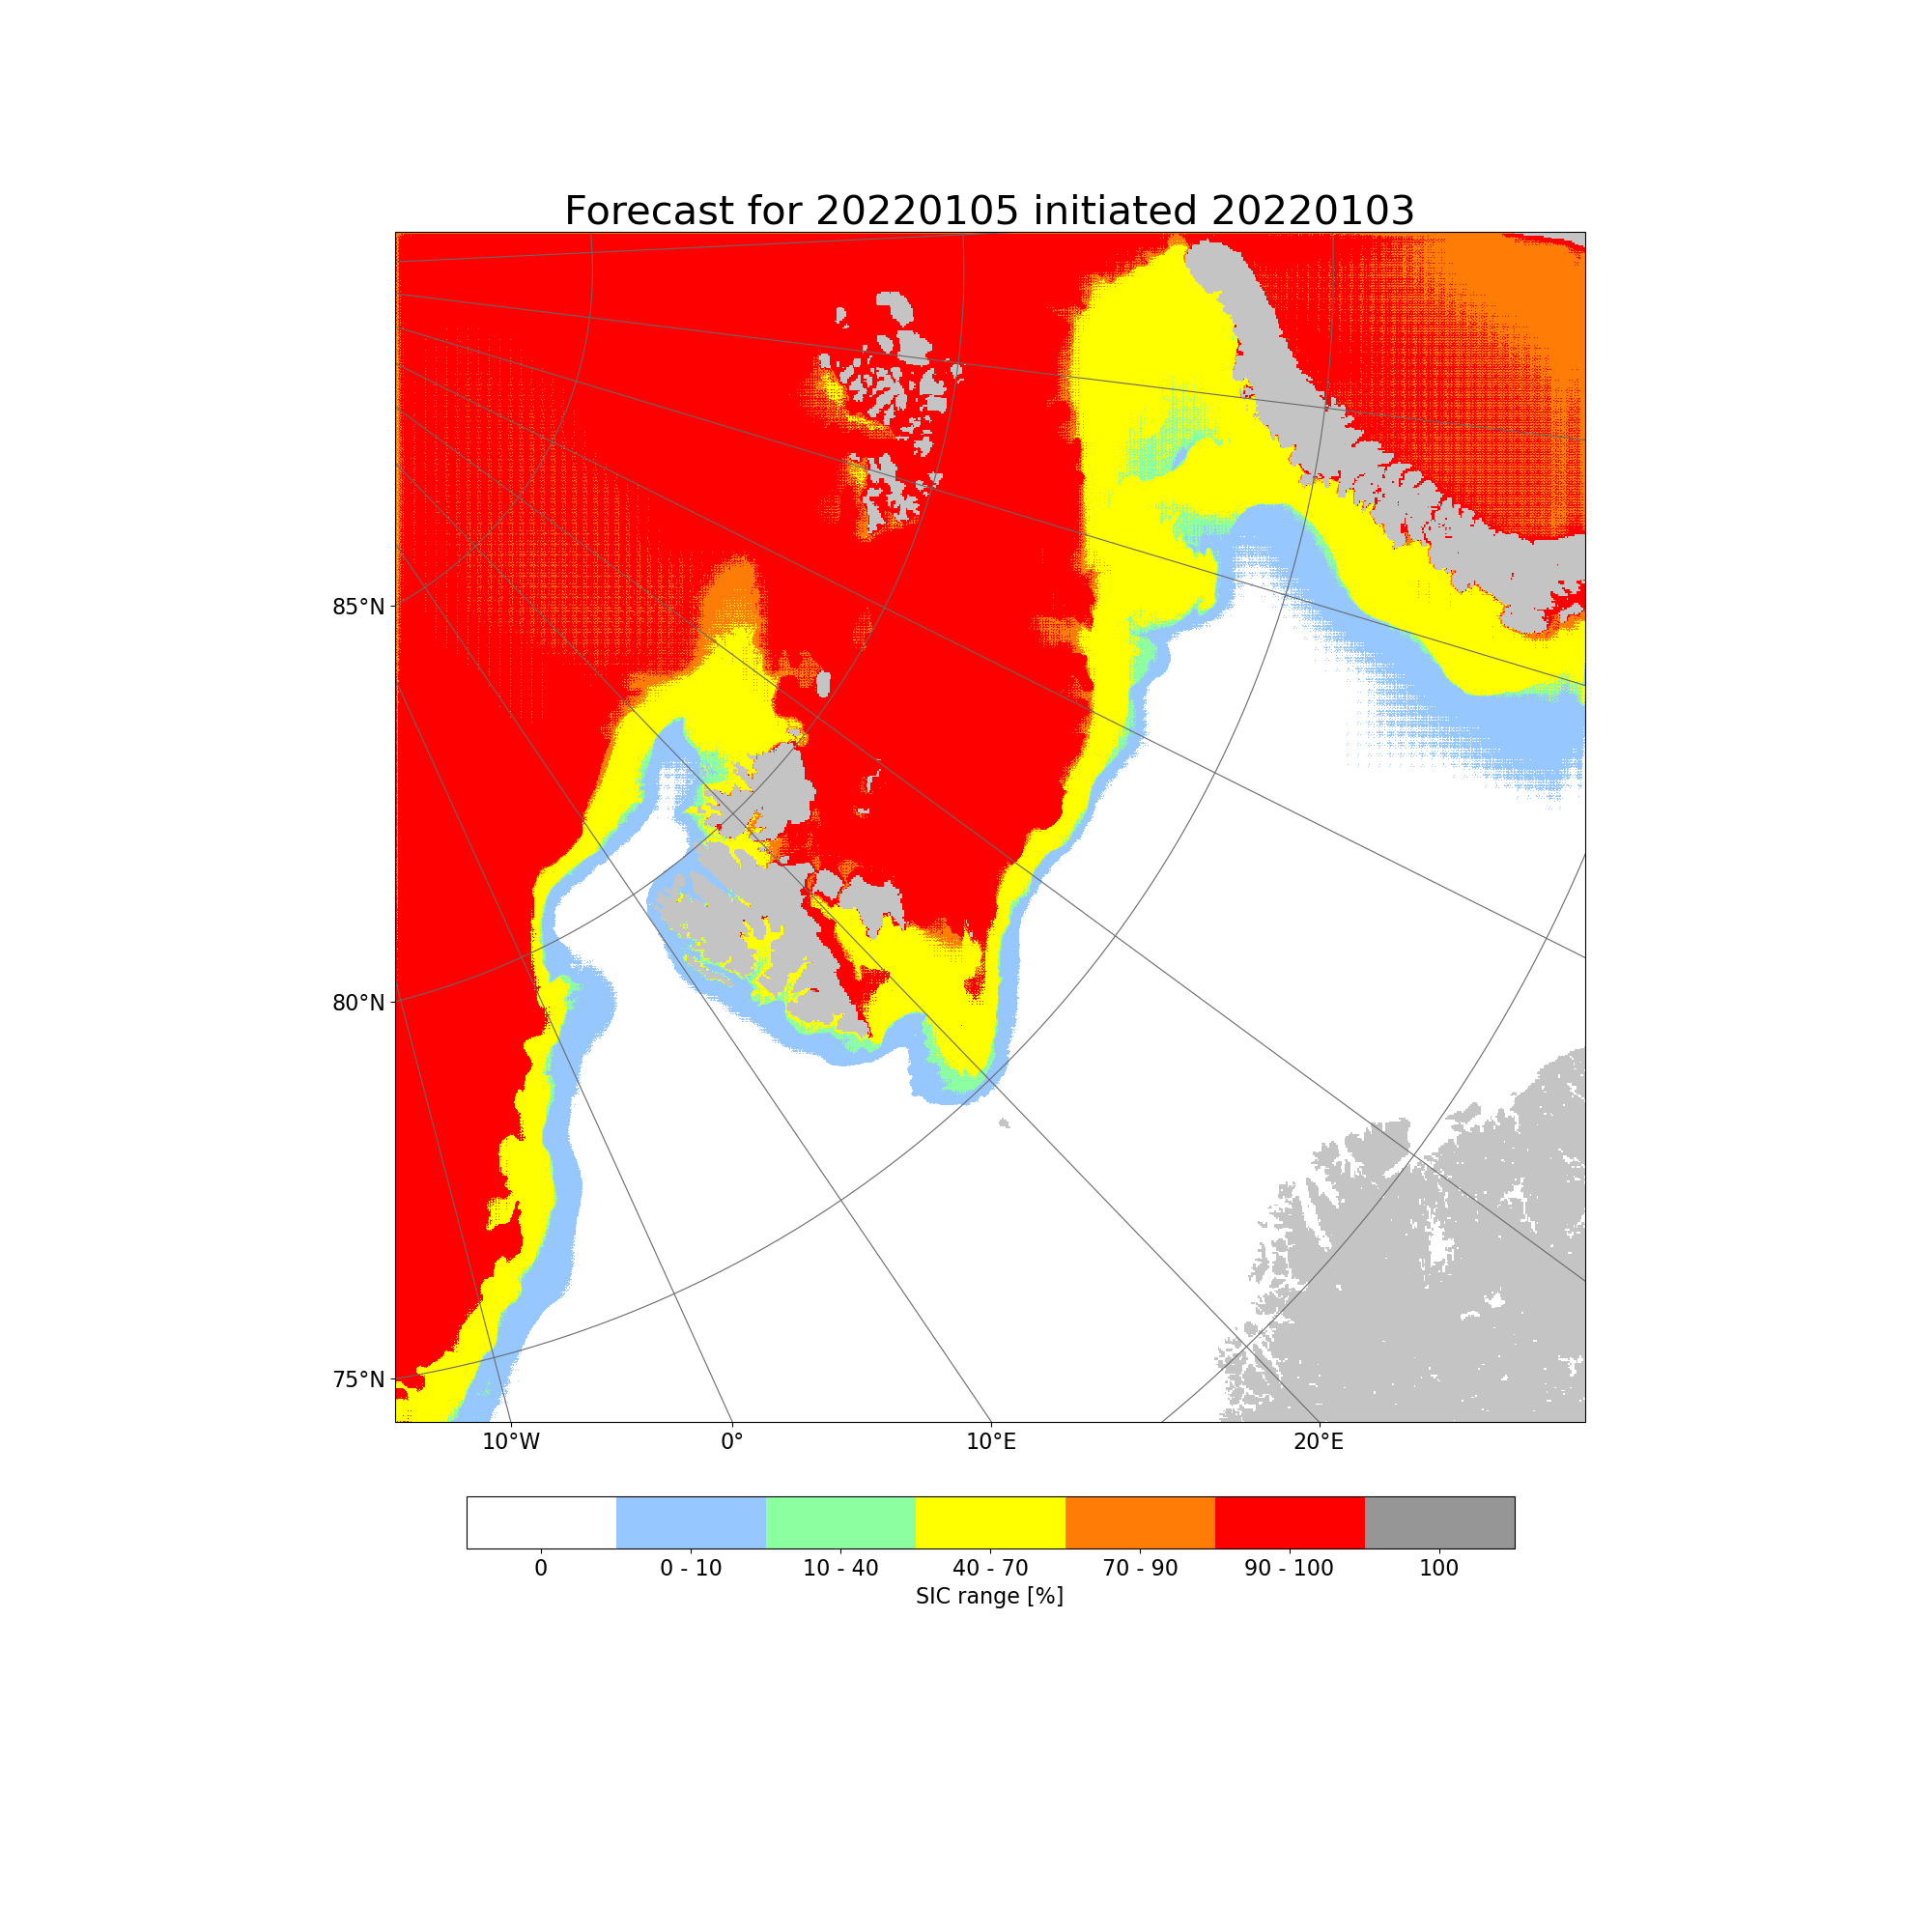
\includegraphics[width=\textwidth]{linear_model_jan}
    \caption{\label{fig:linear_model}Prediction with a two day lead time model, where all non-linear activation functions were replaced with linear mappings. The figure aims at qualitatively showing a prediction made with a linear model.}
\end{figure}

\subsubsection{Modifying the land-sea mask and number of outputs}
\label{sec:modifyhyperparam}
The effect of setting all pixels in the predictor ice chart covered by the land mask as ice-free open water (category 0) was first inspected. When replacing all land covered predictor pixels to ice-free open water, a mean annual NIIEE of 29.72 km was achieved compared to 28.20 km when nearest neighbor interpolation is used. This experiment was motivated to measure the impact of the nearest neighbor interpolated land-sea mask which was inspired by the work of \citet{Wang2017}.

From the description of the cumulative contours in Section \ref{sec:data_targets}, the number of thresholds $k_n$ (Equation \ref{eq:cum_number}) can be reduced such that fewer cumulative contours $c^n$ (Equation \ref{eq:cum_contour}) are targeted. Reducing the number of cumulative contours causes the Deep learning system to output fewer ice categories. The number of target cumulative contours have an effect of the overall loss function propagated throughout the U-Net, with fewer cumulative contour reducing the computed loss (Section \ref{sec:train_env}). This is a direct consequence of the modified computational graph, since the loss backpropagated starting from the decoder is the sum of each individual loss from the output layers. It is also noted that the different sea ice categories have different physical interpretations and associated dynamics, e.g. land fast ice represented by the fast-ice category is assumed to behave differently than the other sea ice categories.

A model was trained with a reduced set of outputs to measure the impact of lowering the number of cumulative contours on model skill. When reducing the number of possible classes in the ice chart, two cumulative contours were modified. First, the $(< 10\%)$ sea ice concentration contour was removed as it is not based on true observations of sea ice (NIS, pers. commun.). Second, the $(\text{fast ice})$ contour was removed as it is expected to represent different dynamics from the other targeted contours. Despite the reduced number of targets, the model was trained equally to other models, and achieved a mean annual NIIEE of 28.61 km compared to 28.20 km when all contours are predicted.

\subsubsection{Connecting validation loss with NIIEE}
\label{sec:connecting_val_loss_with_NIIEE}
Section \ref{sec:train_env} described how model selection is performed, where the model that performs best on the validation dataset (2021) with regards to minimizing the loss is selected. This subsection presents a comparison between the NIIEE and the validation loss.

The IIEE was normalized with respect to a climatological ice edge length derived from ten years of OSI SAF data as described in section \ref{sec:osisafcdr}. When iterating through the validational dataset after an epoch is completed, all validational predictions are used to compute the IIEE with respect to their associated ground truth label. The results are summarized in figure \ref{fig:val_loss_iiee}

\begin{figure}
    \centering
    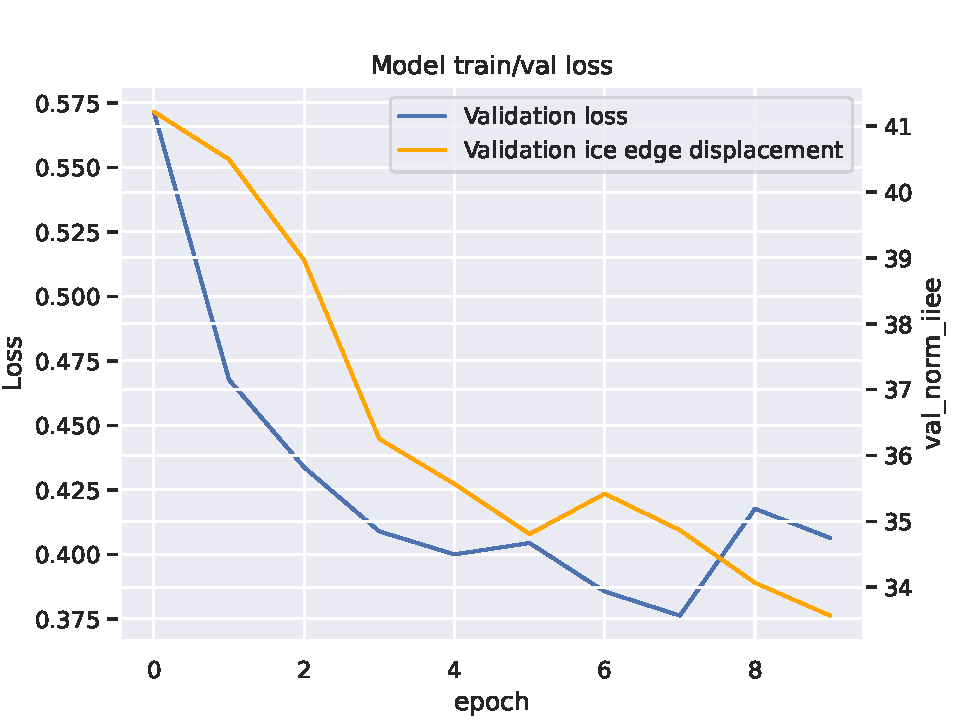
\includegraphics[width=\textwidth]{val_loss_iiee}
    \caption{\label{fig:val_loss_iiee}Validation loss and validation normalized ice edge displacement as a function of epoch. A training environment with a 2 day lead time was used.}
\end{figure}

The correlation between the validation loss and validation normalized ice edge displacement reported in figure \ref{fig:val_loss_iiee} is 0.82. Moreover, training the model for 10 epochs with the previously described IIEE validation scheme took 21 hours, which is a 15 times increase to training time compared to when binary cross-entropy is used for validation. Furthermore a single IIEE validation iteration took 2 hours. Thus it was decided to use the binary cross-entropy as the validation metric for model selection during training.

\biblio
\end{document}